\chapter{Aplikacje klienckie}

Na podstawie analizy statystyk dotyczących podziału rynku aplikacji na platformy, dostępnych na stronie statcounter.com \url{http://gs.statcounter.com/os-market-share/mobile-tablet/worldwide/#monthly-201801-201801-bar} , zdecydowano się na stworzenie 3 klientów systemu The Guard, które pozwolę możliwie największej grupie osób na korzystanie z systemu:
\newline
\newline
\textbullet \space aplikacja mobilna na system Android,\newline
\textbullet \space aplikacja mobilna na system iOS,\newline
\textbullet \space aplikacja webowa.

\section{Funkcje aplikacji}
\paragraph{Logowanie}
Do prawidłowego przejścia do ekranu głównego aplikacji niezbędne jest posiadanie konta. Po rejestracji użytkownika lub po pomyślnym uwierzytelnieniu jeśli konto zostało już wcześniej założone następuje pobranie wszystkich danych użytkownika, jego podłączonych urządzeń i przejście do głównego panelu z dostępem do wszystkich niżej omówionych funkcji. 
\begin{figure}[ht]
	\centering
	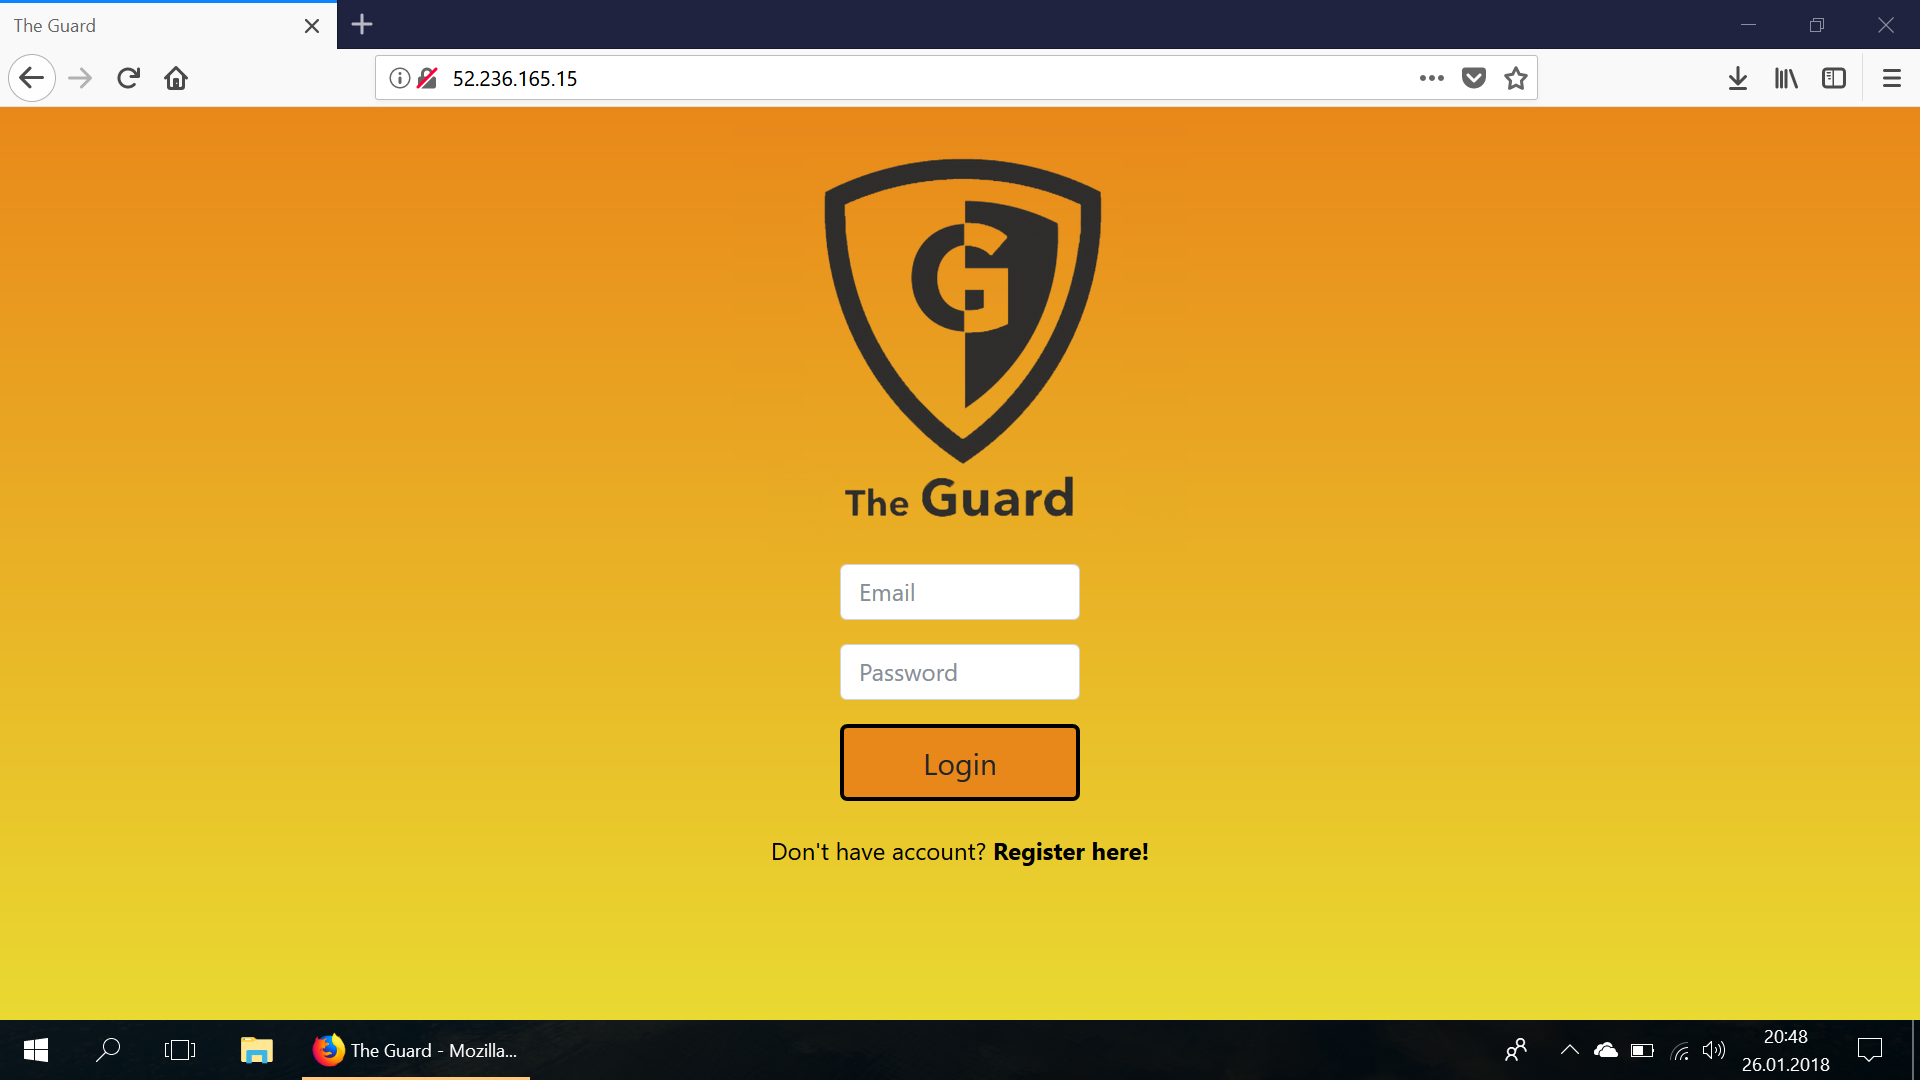
\includegraphics[width=9cm]{web_screenshots/login.png}
	\caption{Strona logowania w aplikacji webowej}
	\label{web_login}
\end{figure}
\paragraph{Monitoring}
Aplikacja pobiera i wyświetla obraz na żywo z zaznaczonego urządzenia podłączonego do konto użytkownika. 
\begin{figure}[ht]
	\centering
	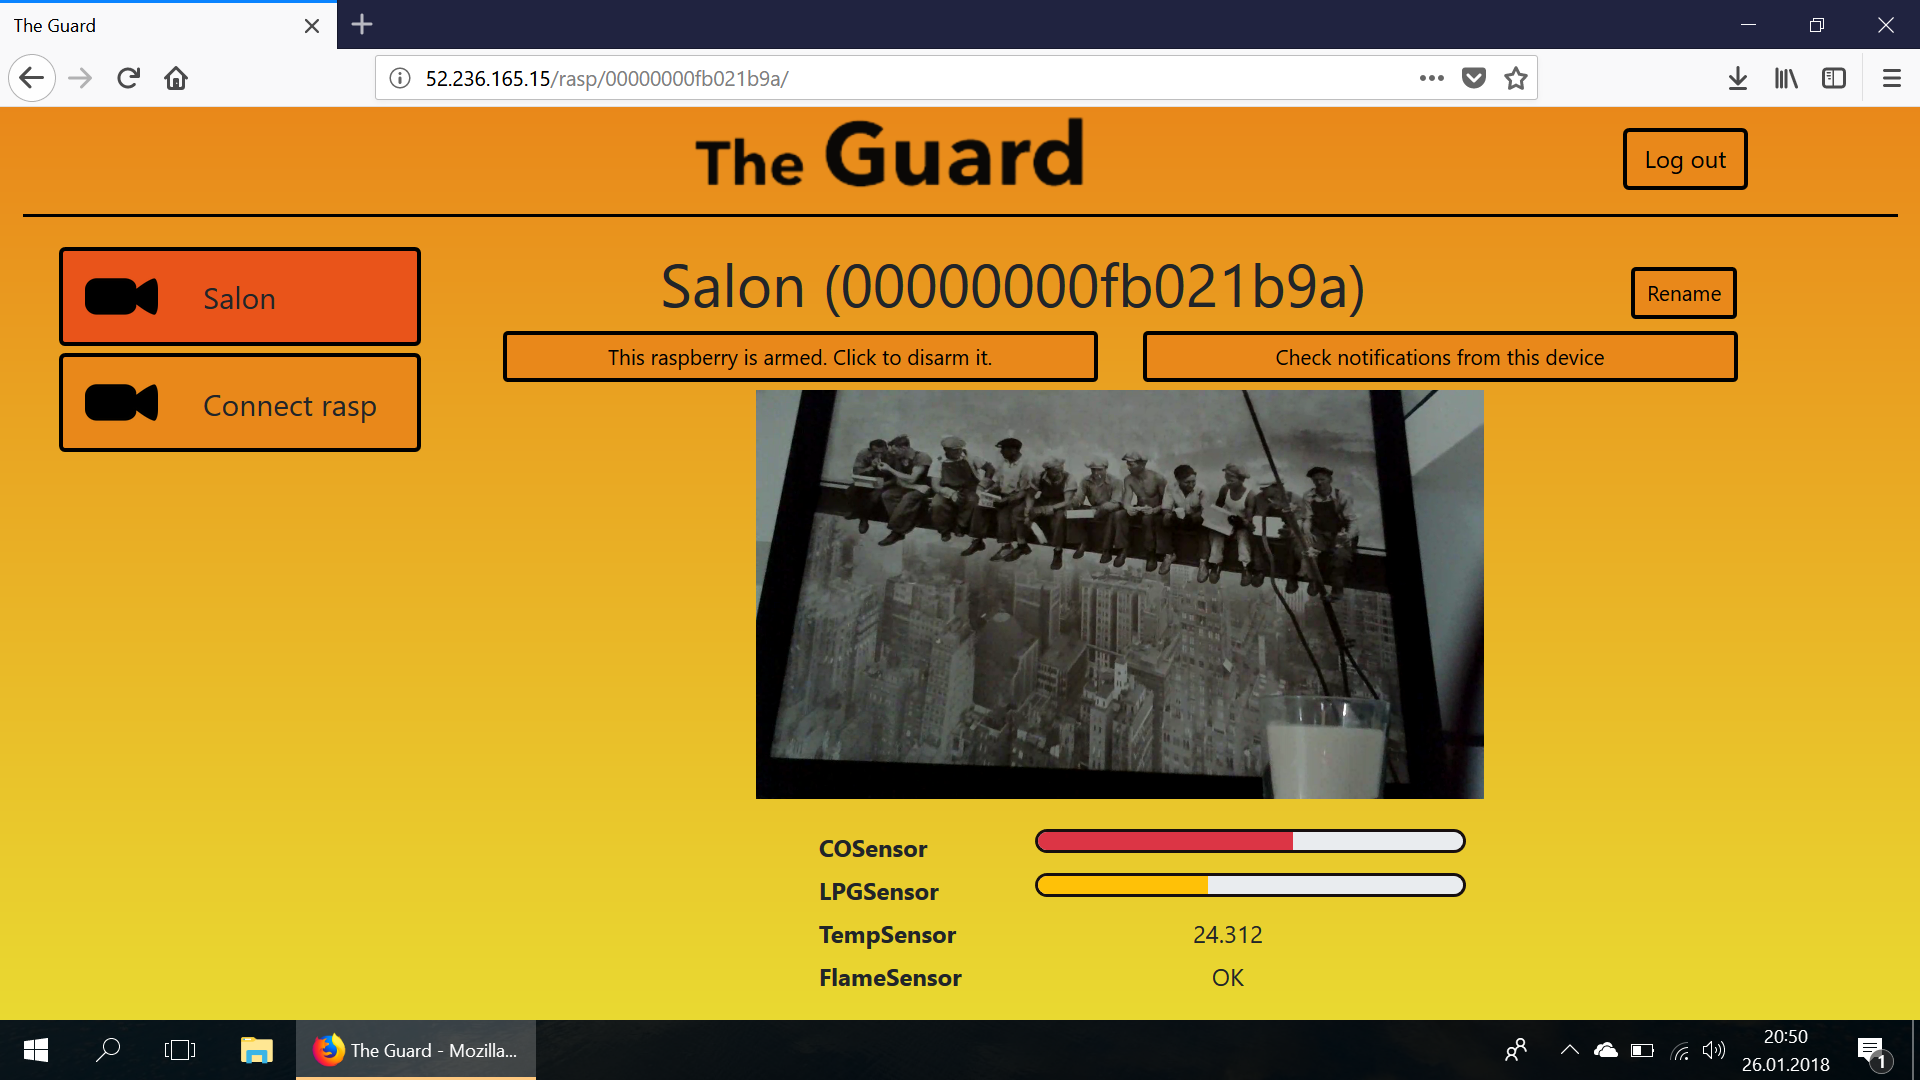
\includegraphics[width=9cm]{web_screenshots/rasp_view.png}
	\caption{Widok konkretnego urządzenia}
	\label{web_rasp_view}
\end{figure}
\paragraph{Status czujników}
Po przejściu do tej sekcji użytkownik otrzymuje bieżące dane z wszystkich czujników z zaznaczonego urządzenia. Na podstawie koloru prezentowanej wartości z czujnika użytkownik może analizować zagrożenie. Kolor zielony reprezentuje bezpieczne odczyty na czujnikach, kolor pomarańczowy średnie, kolor czerwony natomiast oznacza bardzo wysoki poziom niebezpieczeństwa.

\paragraph{Dziennik zdarzeń}
W tej sekcji użytkownik ma dostęp do historii zdarzeń w systemie. 
\begin{figure}[ht]
	\centering
	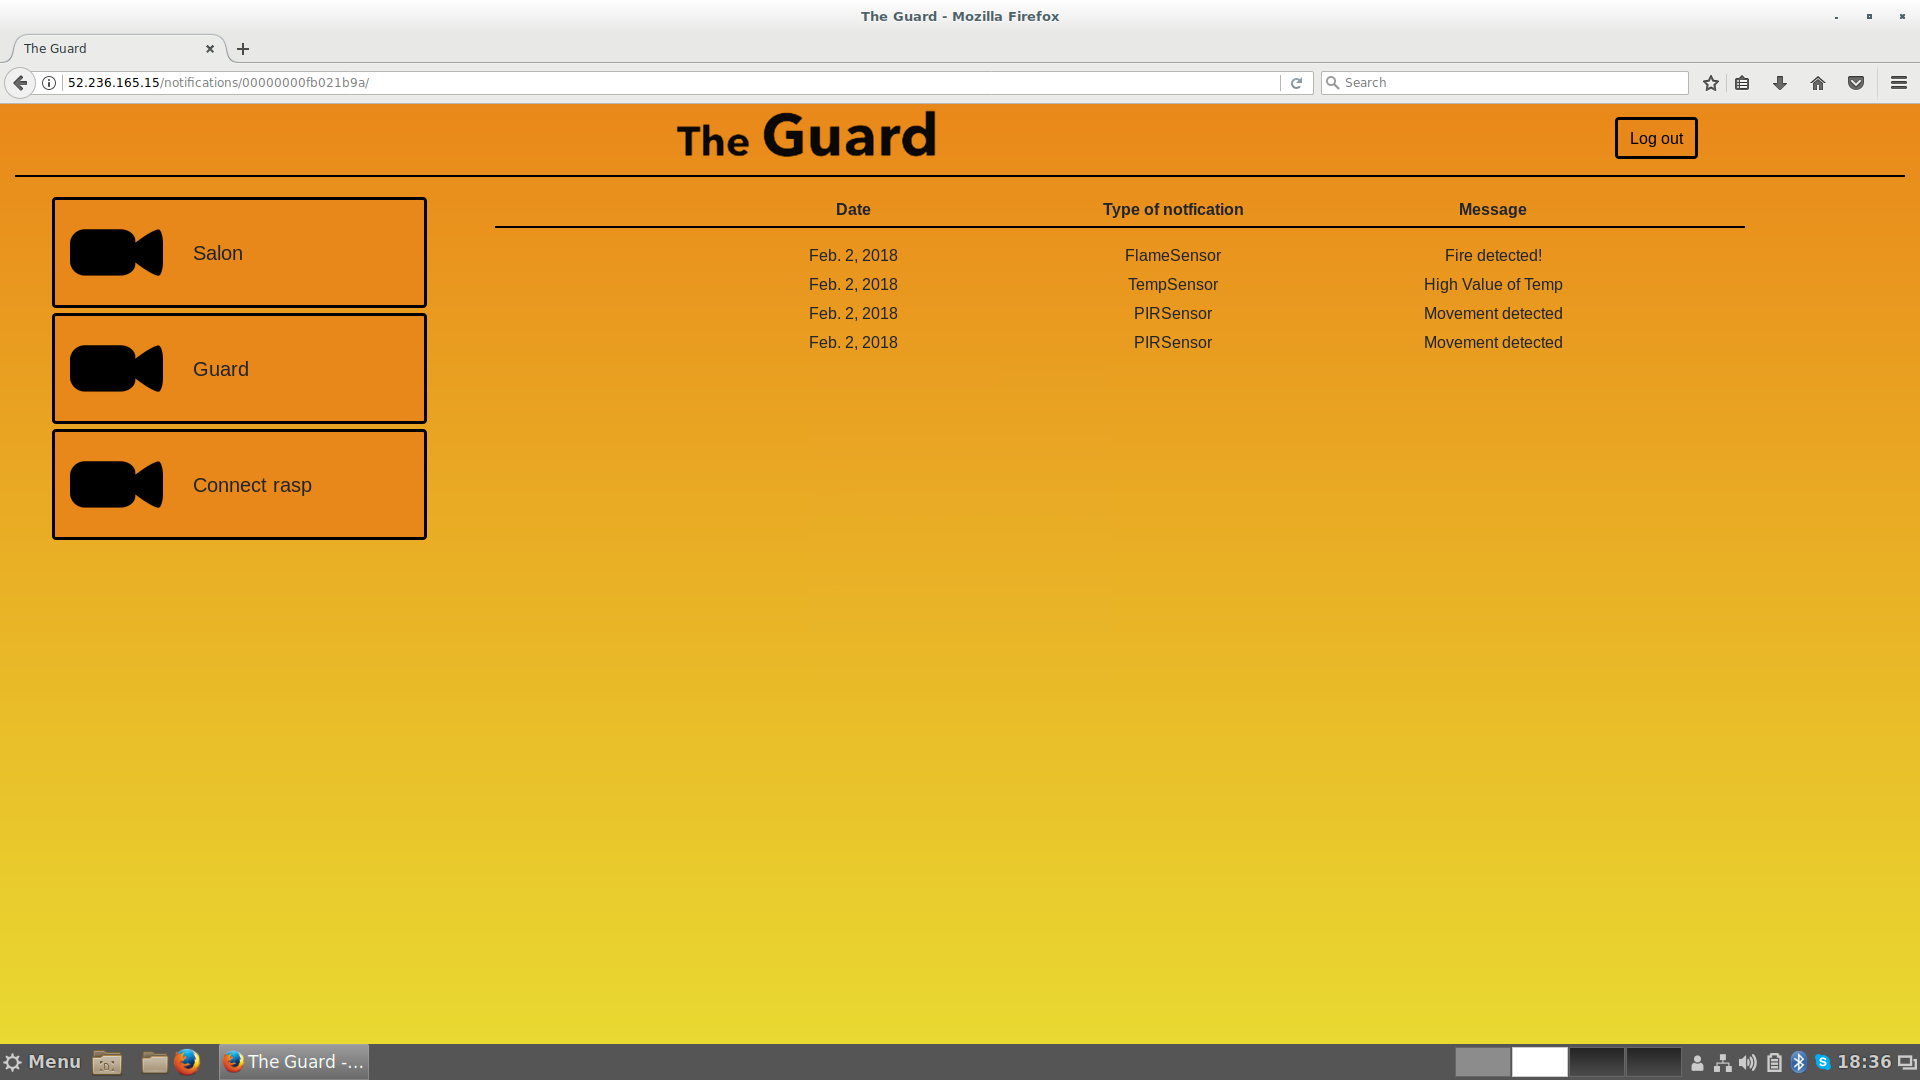
\includegraphics[width=9cm]{web_screenshots/rasp_notifications.png}
	\caption{Panel notyfikacji urządzenia}
	\label{web_rasp_notifications}
\end{figure}
\paragraph{Ostatnie zagrożenia}
Prezentacja ostatniego nagranego zagrożenia. Służy do szybkiego przeglądu ostatniego niebezpieczeństwa i prezentuje ostatni nagrany materiał video. 

\paragraph{Ustawienia urządzenia}
Użytkownik ma możliwość zmiany nazwy urządzenia, które zazwyczaj reprezentuje miejsce, w którym się znajduje. Istnieje również możliwość uzbrojenia i wyłączenia każdego urządzenia. Sprowadza się to do tego, że w przypadku zaznaczenia opcji "Disarmed"  użytkownik nie otrzyma kolejnych notyfikacji o zagrożeniach. Opcja ta może okazać się przydatna w momencie uszkodzenia któregoś z modułów i tym samym błędnych danych wysyłanych z czujników.
\begin{figure}[ht]
	\centering
	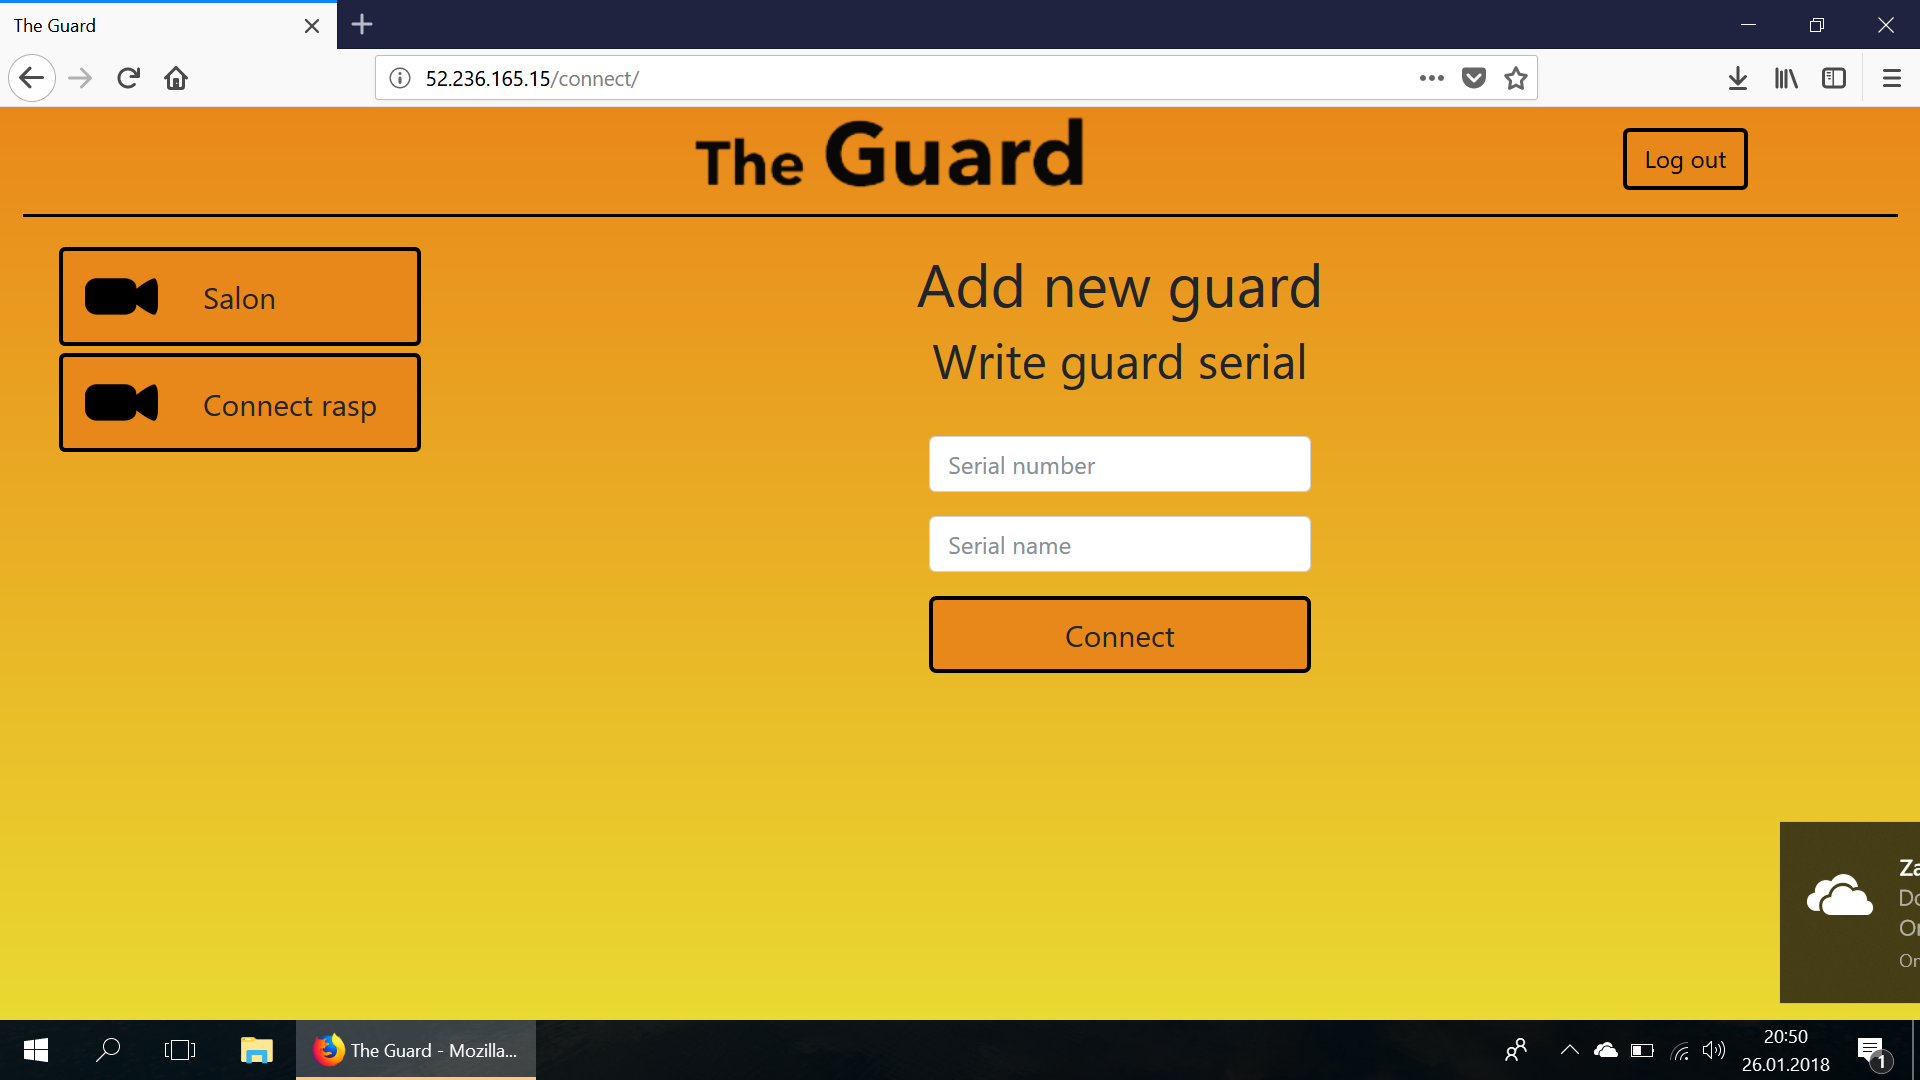
\includegraphics[width=9cm]{web_screenshots/add_rasp.png}
	\caption{Panel rejestracji nowego urządzenia}
	\label{web_register}
\end{figure}
\begin{figure}[ht]
	\centering
	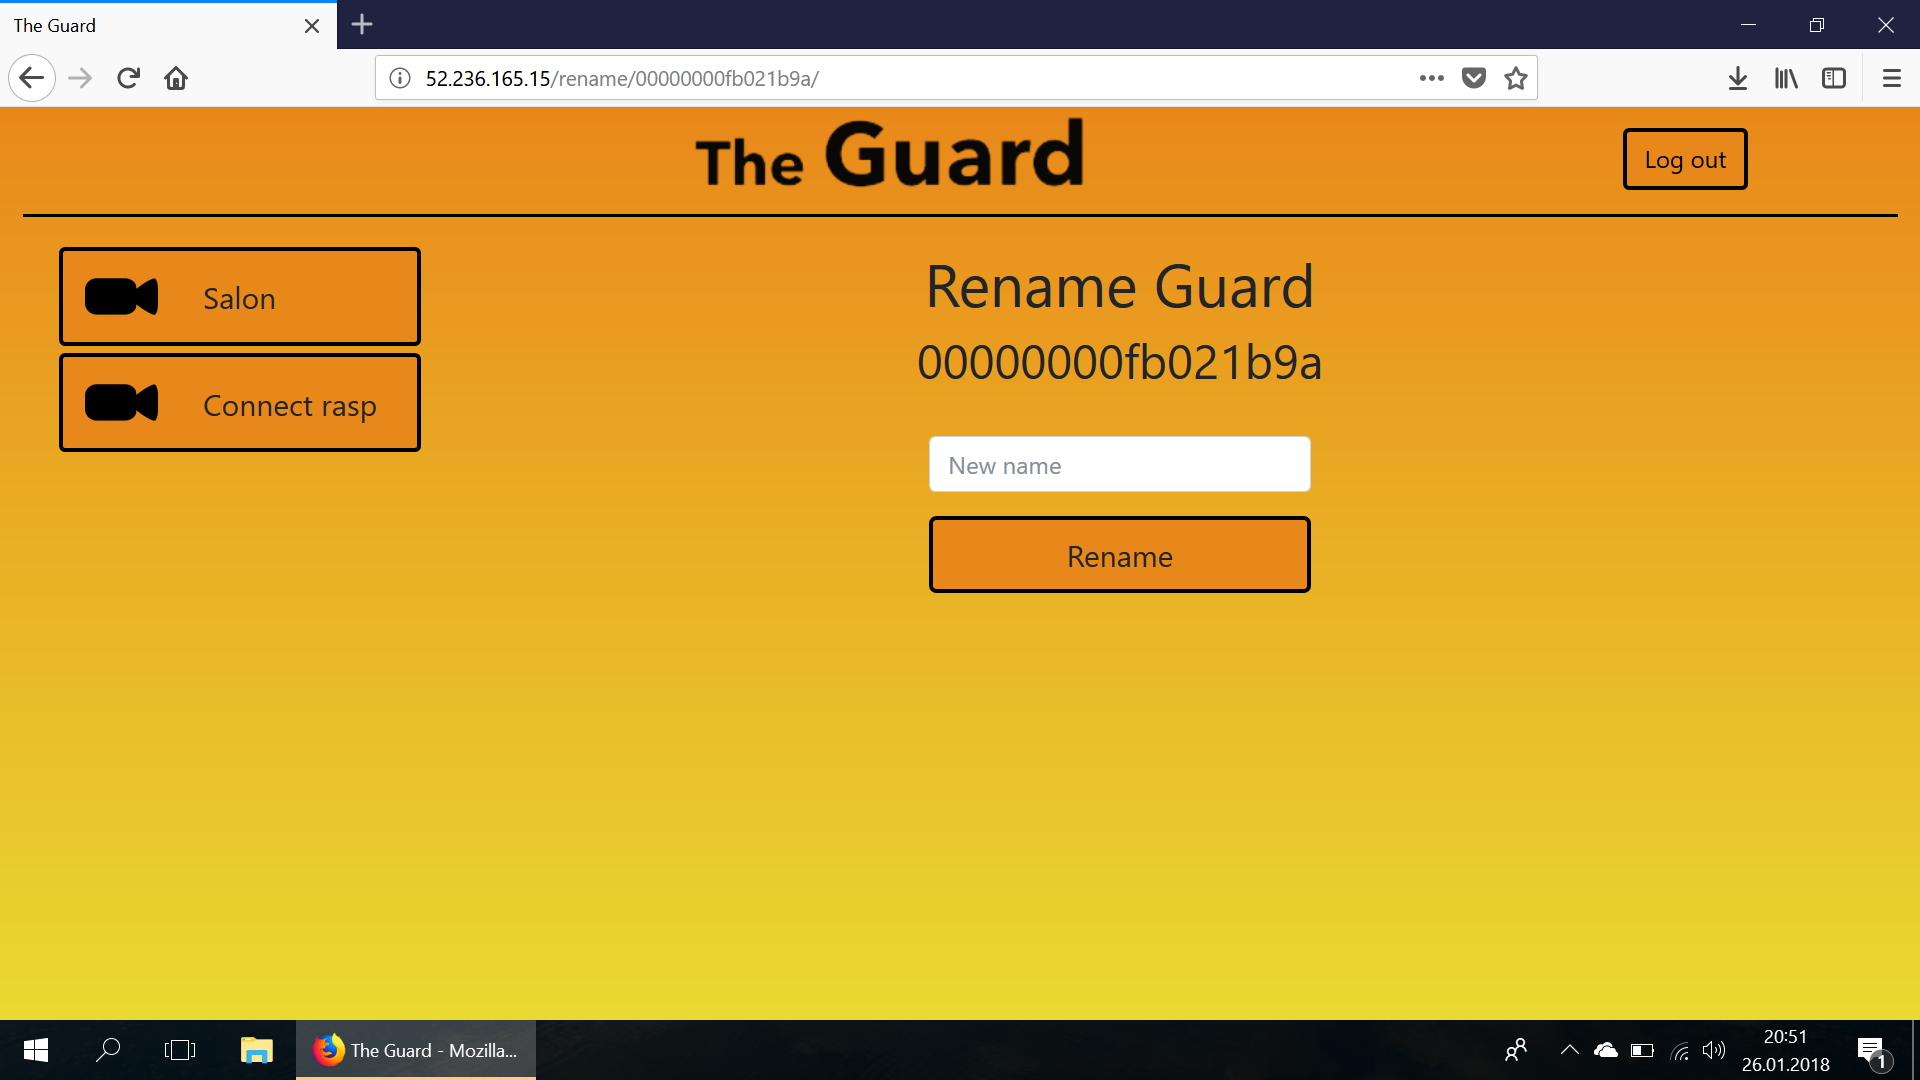
\includegraphics[width=9cm]{web_screenshots/rasp_rename.png}
	\caption{Panel zmiany nazwy urządzenia}
	\label{web_rasp_rename}
\end{figure}

\section{Aplikacja Android}
\subsection*{Wybór narzędzi}
Do stworzenia aplikacji mobilnej na system Android użyto języka Kotlin - języka stworzonego przez firmę JetBrains, który 17 maja 2017 roku został uznany przez Google jako oficjalny język programowania aplikacji na platformę Android.\footnote{\url{https://twitter.com/Android/status/864911929143197696}}
Kotlin ściśle współegzystuje z kodem stworzonym w Javie i w przypadku Androida jest kompilowany do kodu JVM.

Skorzystano ze środowiska Android Studio w wersji 3.0.1, do automatyzacji budowy projektu został wykrozystany Gradle w wersji 4.1.

Aplikacja skierowana jest na urządzenia z systemem Android od wersji Lollipop 5.0 (o numerze SDK większym niż 20), który został wydany 12.12.2014 r. Ograniczenie wersji spowodowane jest możliwością użycia bardziej zaawansowanych komponentów, niedostępnych dla niższych wersji. W styczniu 2018 r. oficjalne statystyki informują o tym, że około 80,7 \% wszystkich urządzeń z systemem Android na świecie ma wersję 5.0 lub wyższą.

\subsection*{Architektura}
Aplikacja The Guard dla systemu Android została stworzona zgodnie z założeniami architektury Model View Presenter. Architektura MVP zakłada rozdzielenie kodu źródłowego aplikacji na 3 kategorie:

\textbullet \space "Model", czyli kod odpowiedzialny za logikę biznesową, połączenie z serwerem i złożone operacje,\newline
\textbullet \space "View", czyli kod odpowiedzialny wyłącznie za poprawne wyświetlanie przygotowanych informacji,\newline
\textbullet \space "Presenter", czyli kod odpowiedzialny za przygotowanie informacji otrzymanych z warstwy model do wyświetlenia w warstwie View.\newline

sNajwiększą zaletą architektury MVP jest możliwość wygodnego testowania logiki aplikacji (w warstwie Presenter) oraz zastosowanie programowania reaktywnego przy użyciu biblioteki RxKotlin.
Warstwy komunikują się między sobą w sposób reaktywny - przy użyciu strumieni wydarzeń. Przykładowo klasa warstwy Presenter odpowiedzialna za wyświetlanie obrazu z kamery wykorzystuje klasę warstwy Model do asynchronicznej komunikacji z API.

\subsection*{Funkcje i interfejs użytkownika}
Aplikacja została zaprojektowana zgodnie z wytycznymi Material Design\footnote{Learning Material Design: Master Material Design and create beautiful, animated interfaces for mobile and web applications, Kyle Mew, Packt Publishing 2015}.
Do nawigacji po funkcjach aplikacji służy panel na dole ekranu - "Bottom Bar".
Zanim będzie on widoczny, użytkownik musi najpierw zalogować się (lub zarejestrować) przy użyciu adresu email oraz hasła.

\paragraph{Logowanie}

\begin{figure}[ht]
	\centering
	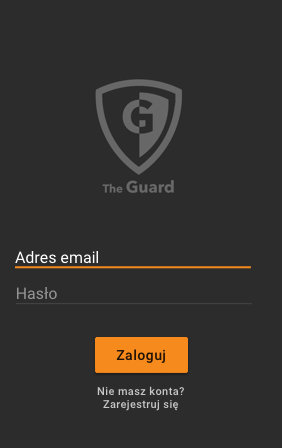
\includegraphics[width=6cm]{Logowanie}
	\caption{Ekran logowania do aplikacji}
\end{figure}

Użytkownik loguje się do aplikacji przy użyciu adresu email oraz hasła. Dane te trafiają do Firebase Authotizdtio

\subsection*{Integracje}
Opis połączenia aplikacji z Firebase, Fabric i innymi bibliotekami.

\begin{figure}[ht]
    \centering
    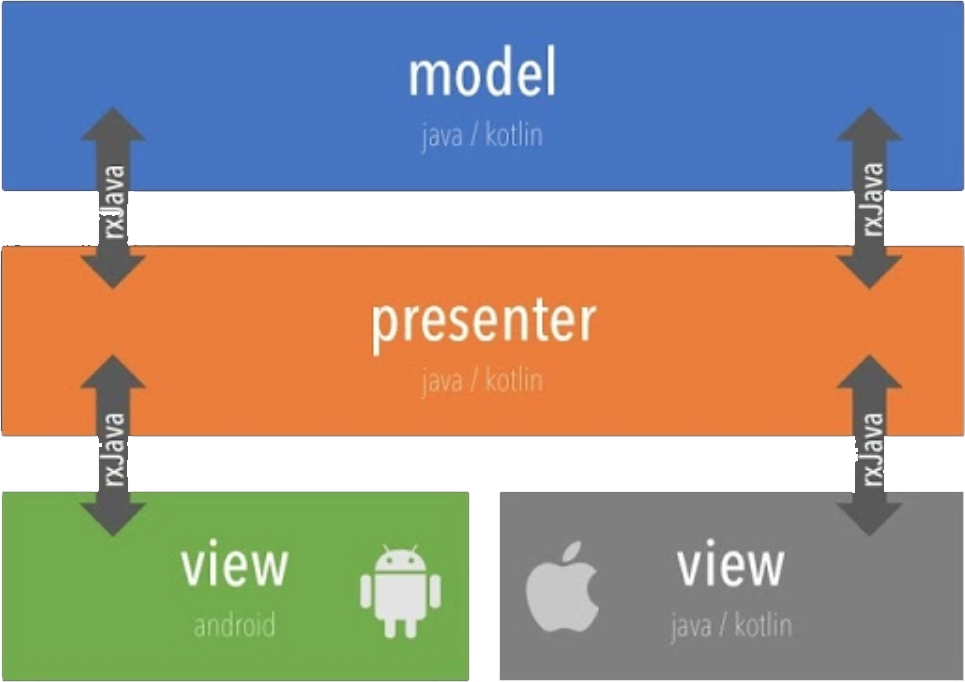
\includegraphics[width=9cm]{ios_screenshots/android_architecture.png}
    \caption{Architektura MVP}
\end{figure}

\section{Aplikacja iOS}
Aplikacja przeznaczona jest na urządzenia z systemem operacyjnym iOS od wersji 10.0. 
Nie wspiera ona wcześniejszych wersji ze względu na nowe funkcje, które Apple wprowadziło wraz z pojawieniem się iOS 10.0 (m.in. klasa UNUserNotificationCenter). Jednak 93\% wszystkich obecnych użytkowników tego systemu(rys. 5.1) jest w stanie zainstalować oprogramowanie a liczba ta stale rośnie. Aplikacja wspiera zarówno telefony komórkowe iPhone jak i tablety iPad. 
\begin{figure}[ht]
	\centering
	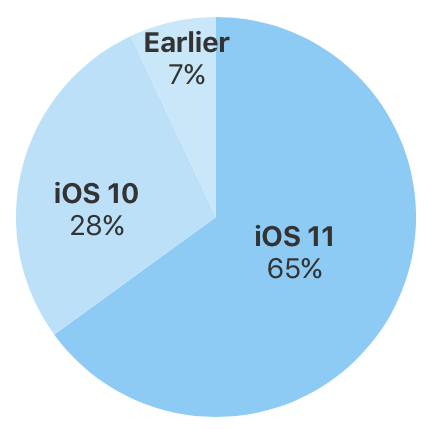
\includegraphics[width=4cm]{ios_screenshots/iOSstat.png}
	\caption{Udziały wersji systemu iOS z 18.01.2018 \protect\cite{iosversions}}
\end{figure}
Napisana w stosunkowo nowym języku Swift (zaprezentowany przez Apple w 2014 roku) w oparciu o architekturę MVC (Model-View-Controller) wykorzystując przy tym programowanie reaktywne i funkcjonalne. Aplikacja powstała w programie Xcode. Programowanie reaktywne zrealizowano przy pomocy biblioteki RxSwift. Ten paradygmat programowania związany jest z pojęciem obserwatora i sekwencji obserwowalnych. Każdy obserwator wywołując funkcję 'subscribe' na elemencie obserwowalnym otrzymuje informację o każdej zmianie na tym obiekcie. RxSwift wykorzystano m.in w celu wznowienia streamu obrazu z kamery w momencie przejścia aplikacji z trybu pracy w tle do trybu aktywnego. Oznacza to, że po wyjściu z aplikacji i po ponownym jej uruchomieniu tracono obraz ze streamu. Przyczyną jest polityka Apple, która nie zaleca aby aplikacje pracowały w tle i domyślnie wyłącza każdą taką aktywność. Ma to na celu przedłużenie żywotności baterii i optymalizacji całego systemu poprzez ograniczenie ilości zajmowanych zasobów \cite{backgroundmodes}.  Oczywiście istnieje możliwość włączenia pracy w tle, jednakże konieczne jest aktywowanie trybu "Background Modes" i zaznaczenie konkretnej aktywności, którą chcielibyśmy wykonywać. Lista dozwolonych czynności możliwych do realizacji jest jednak ograniczona (rys. 5.2). 
\begin{figure}[ht]
	\centering
	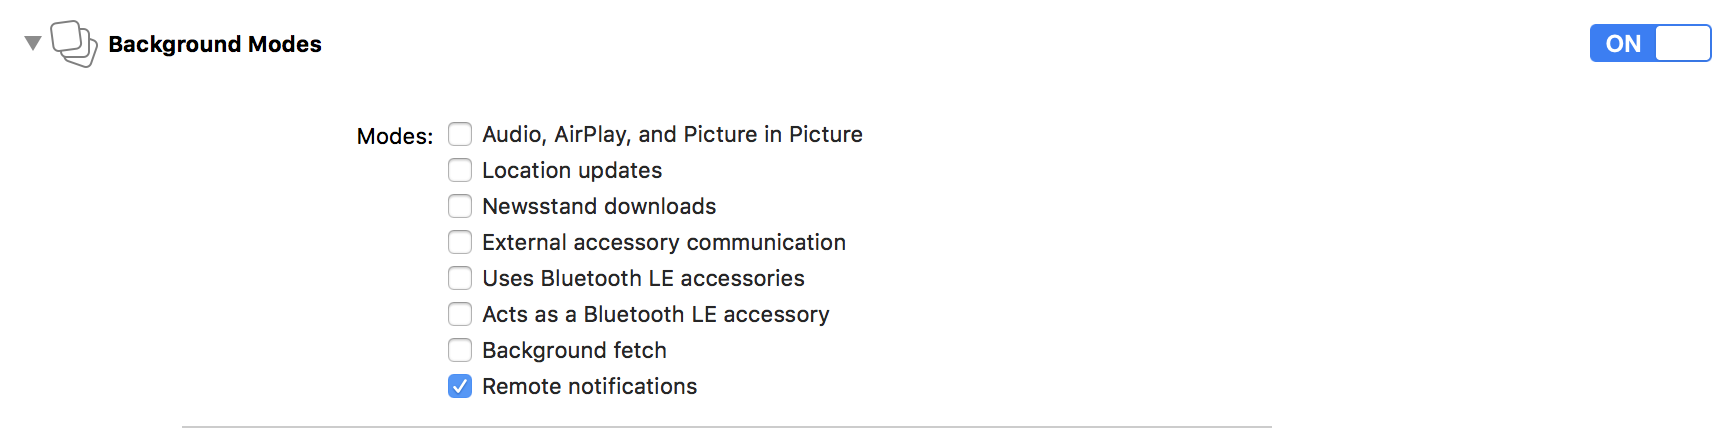
\includegraphics[width=10cm]{ios_screenshots/backgroundModes.png}
	\caption{Tryby pracy w tle [źródło własne]}
\end{figure}
Próba oszustwa i wykonywania innej pracy w tle niż zaznaczona zostanie wychwycona w procesie weryfikacji przed jej publikacją na platformie Apple Store. Dzięki programowaniu reaktywnemu problem wznowienia podglądu obrazu został rozwiązany co prezentuje poniższy kod:
\begin{verbatim}
let appDelegate = UIApplication.shared.delegate as! AppDelegate
        appDelegate.inBackground.asObservable().subscribe(onNext: { (value) in
            if let streamView = self.streamView {
                if let player = self.currentPlayer {
                    if value == false {
                        self.streamVideoFrom(urlString: self.currentUrlString!)
                        print("Enter foreground")
                    } else {
                        print("Enter background")
                        streamView.layer.sublayers?.forEach({ (layer) in
                            layer.removeFromSuperlayer()
                        })
                    }
                }
            }
        }).disposed(by: disposeBag)
\end{verbatim}
Zmienna 'inBackground', która jest zmienną obserwowalną, ustawiana jest w oddzielnej klasie AppDelegate (klasa, która zapewnie poprawną interakcję z systemem iOS) na wartość true w chwili przejścia do trybu pracy w tle i na wartość false w przeciwnym wypadku. Klasa, w której wywoływany jest funkcja 'subscribe' jest obserwatorem tej zmiennej. Kod wewnątrz funkcji subscribe uruchamiany jest przy każdej zmianie wartości 'inBackground' i wznawia ponownie stream po każdym ponownym uruchomieniu programu.
"Programowanie funkcjonalne natomiast polega na traktowaniu funkcji jako obiektu. Oznacza to, że mogą być one zapisywane, kopiowane i przekazywane tak samo jak wszystkie inne obiekty. Mogą być używane jako parametry innych funkcji." \cite[p.~172]{proswift}. Wykorzystane są w miejscach gdzie konieczne jest przekształcanie danych:
\begin{verbatim}
lastNotification = notifications.array.sorted(by: { (n1, n2) -> Bool in
	n1.date > n2.date 
}).filter({ (notif) -> Bool in return notif.type == "PIRSensor"}).first
\end{verbatim}
Na tablicy z notyfikacjami zastosowano szereg kolejnych funkcji: posortowano je malejąco według daty, przefiltrowano w taki sposób aby wybrać tylko te o typie 'PIRSensor' czyli te pochodzące z czujnika ruchu. Na sam koniec wybrano tylko jeden pierwszy element z wybranych i wynik wpisano do zmiennej lastNotification. Ważne jest, że każda kolejna wywoływana funkcja np. filter, odbiera wynik poprzedniej. 

Strukturę kodu (rys. 5.3) podzielono na kilka osobnych, logicznych części. Folder Firebase zawiera model bazy danych czujników, które zapisane są na serwerach Firebase. W folderze GuardManager znajdują się elementy odpowiedzialne za komunikację REST-ową z serwerem Django i modele bazy danych znajdującej się na naszym serwerze. Folder Views jest zbiorem widoków, które wczytywane są w zależności, w której sekcji się znajdujemy (opis sekcji niżej). ViewController.swift jest głównym kontrolerem zarządzającym widokami i modelami. Odpowiada za załadowanie odpowiedniego widoku i prezentację danych z odpowiedniej sekcji. W folderze GuardianAppTests napisane zostały testy jednostkowe, które sprawdzają poprawność przekształcania danych typu JSON (odpowiedź serwera) do obiektów zdefiniowanych w folderze GuardManager/Models. Klasy, których nazwy kończą się na Manager oznaczają obiekty typu Singleton. Celem takiego wzorca jest zapewnienie istnienia tylko jednej instancji w całej aplikacji i globalnego dostępu do tego obiektu. GuardManager, który odpowiada za pobieranie danych z bazy danych - taki obiekt nie powinien być utworzony więcej niż jeden raz, gdyż wszystkie klasy, które z niego korzystają nie potrzebują kolejnych instancji tej klasy. W ten sposób zapewniono, że zawsze odwołujemy się do tego samego obiektu.
\begin{figure}[ht]
	\centering
	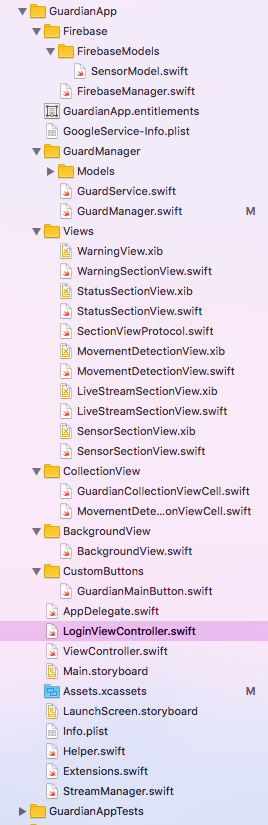
\includegraphics[width=4cm]{ios_screenshots/iOSstructure.png}
	\caption{Struktura aplikacji [źródło własne]}
\end{figure}
Instalacja zewnętrznych bibliotek odbywa się za pomocą CocoaPods. Jest to menadżer zależności dzięki któremu szybko możemy wyszukać i zainstalować wymagane oprogramowanie. Wszystkie użyte zależności przedstawiono poniżej: 
\begin{verbatim}
  pod 'Moya'
  pod 'MBProgressHUD', '~> 1.0'
  pod 'RxSwift',    '~> 4.0'
  pod 'RxCocoa',    '~> 4.0'
  pod 'IHKeyboardAvoiding'
  pod 'Moya-SwiftyJSONMapper'
  pod 'Firebase/Core'
  pod 'Firebase/Messaging'
  pod 'Firebase/Auth'
  pod 'Firebase/Database'
  pod 'M13ProgressSuite'
\end{verbatim}
Moya używana jest do asynchronicznej REST-owej komunikacji z serwerem Django. SwiftyJSONMapper przydatna okazuje się do przekształcenia odpowiedzi serwera w postaci JSON do wcześniej zdefiniowanego modelu. MBProgressHUD umożliwia wyświetlanie ekranu ładowania podczas pobierania informacji z serwera. RxSwift i RxCocoa to biblioteki do programowania reaktywnego. Moduły Firebas/Core itp. służą do komunikacji z serwerami Firebase. Ostatni 'pod M13ProgressSuite' służy do rysowania wykresów i animowanych elementów graficznych w systemie iOS.
Po uruchomieniu aplikacji pierwszym widokiem jest ekran logowania i rejestracji użytkowników (rys 5.4). 
\begin{figure}[ht]
	\centering
	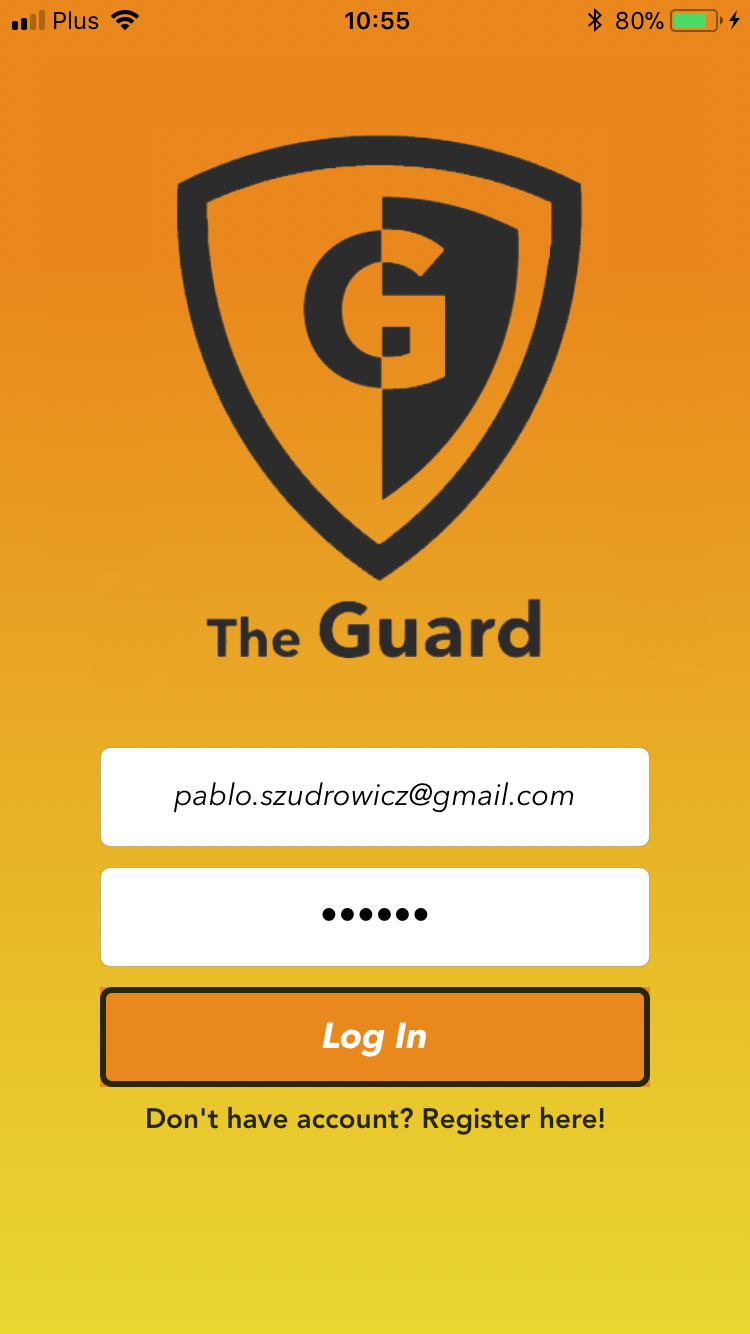
\includegraphics[width=5cm]{ios_screenshots/login.png}
	\caption{Ekran logowania [źródło własne]}
\end{figure}
Po prawidłowym uwierzytelnieniu użytkownika uzyskiwany jest dostęp do głównego widoku aplikacji. W górnej części możliwy jest wybór 5 sekcji:
sekcja czujników, sekcja historii notyfikacji, sekcja ostatnich zagrożeń przy wykryciu ruchu, sekcja monitoringu na żywo, sekcja ustawień. Wszystkie te sekcje dotyczą konkretnego urządzenia wybranego na pasku u dołu ekranu. Funkcje każdej z nich zostały opisane w rozdziale 6.1, tutaj zostaną zaprezentowane jedynie szczegóły implementacyjne i zrzuty ekranów z wersji na iOS. Przy pierwszym uruchomieniu nie istnieje żadne urządzenie przypisane do naszego konta użytkownika. Aby dodać pierwsze i kolejne stacje, od których chcemy otrzymywać notyfikacje o zagrożeniach a także śledzić i monitorować informacje z czujników należy wybrać przycisk "New" z plusikiem w dolnej części ekranu. Pojawi się okno z prośbą o wpisanie numeru identyfikującego urządzenie. Po chwili dodany "Guard" będzie widoczny w na liście.


\paragraph{Sekcja czujników:}
Jest to jedna z najważniejszych sekcji aplikacji (rys 5.5).  Otrzymuje ona dane z czujników w czasie rzeczywistym i prezentuje je użytkownikowi. Implementacja funkcjonalności prezentowania zagrożenia na konkretnym czujniku przy użyciu kolorów zrealizowana została przy pomocy modelu HSV, który w przeciwieństwie do RGB pozwala na bardzo proste przejście z jednego koloru do kolejnego poprzez zmienę tylko jednego parametru. Zmieniając parametr Hue zmieniamy barwę przy stałym nasyceniu i jasności. Wartość tego parametru równa 120\textdegree{} odpowiada kolorowi zielonemu, kolor czerwony to 0\textdegree{}. Przekształcając wartość otrzymaną z czujników, która jest z zakresu [0-1] na wartość z przedziału [120-0] otrzymano wspomniany efekt. 
Poniżej przedstawiono fragment konwersji danych z czujników na kolor w modelu HSV, gdzie zmienna sensors[0] reprezentuje czujnik LPG.
\begin{verbatim}
UIColor(hue: CGFloat(0.33 - (sensors[0].value * 0.33)),
saturation: 1, brightness: 1, alpha: 1)
\end{verbatim}
\begin{figure}[ht]
	\centering
	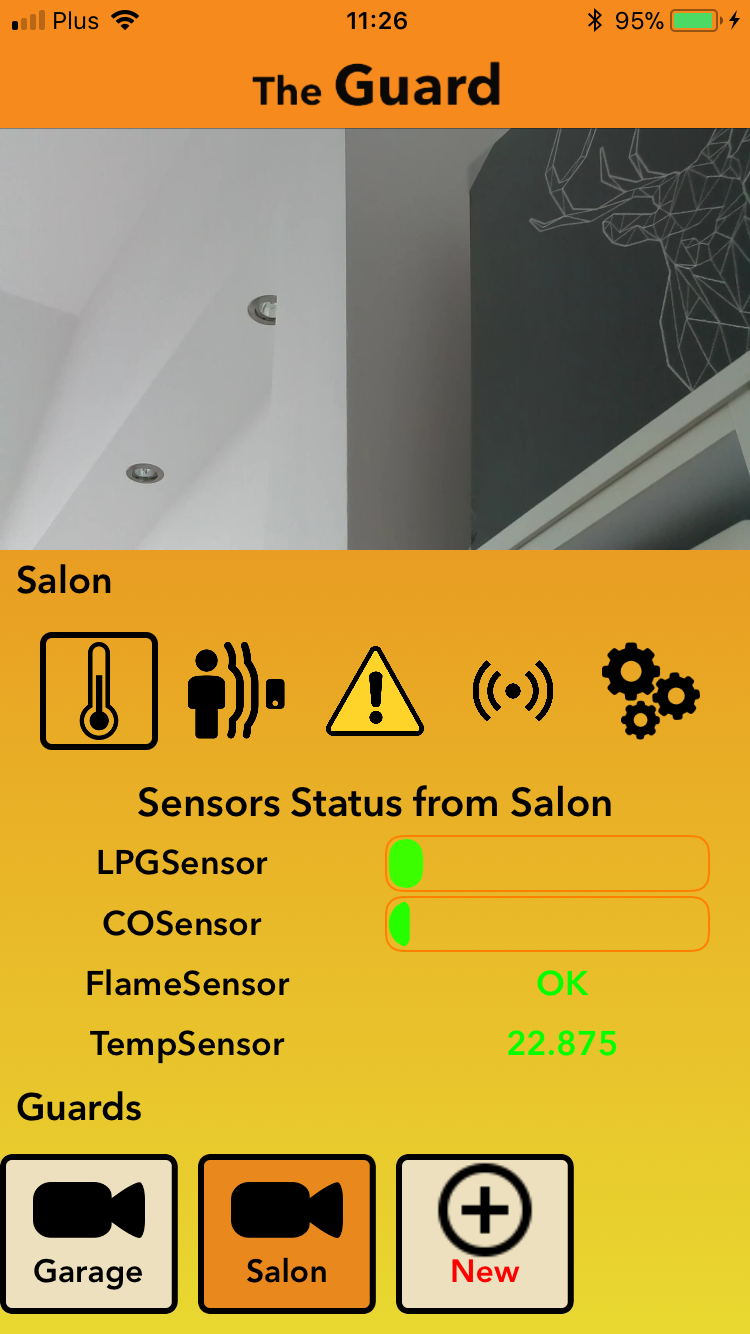
\includegraphics[width=5cm]{ios_screenshots/sensors.png}
	\caption{Sekcja czujników [źródło własne]}
\end{figure}
\paragraph{Sekcja historii notyfikacji:}
Po zaznaczeniu daty reprezentującej moment wystąpienia zagrożenia i wybraniu przycisku 'preview' prezentowana jest informacja o miejscu niebezpieczeństwa i jego rodzaju. (rys 5.6).
\begin{figure}[ht]
\centering
\begin{minipage}{.4\linewidth}
    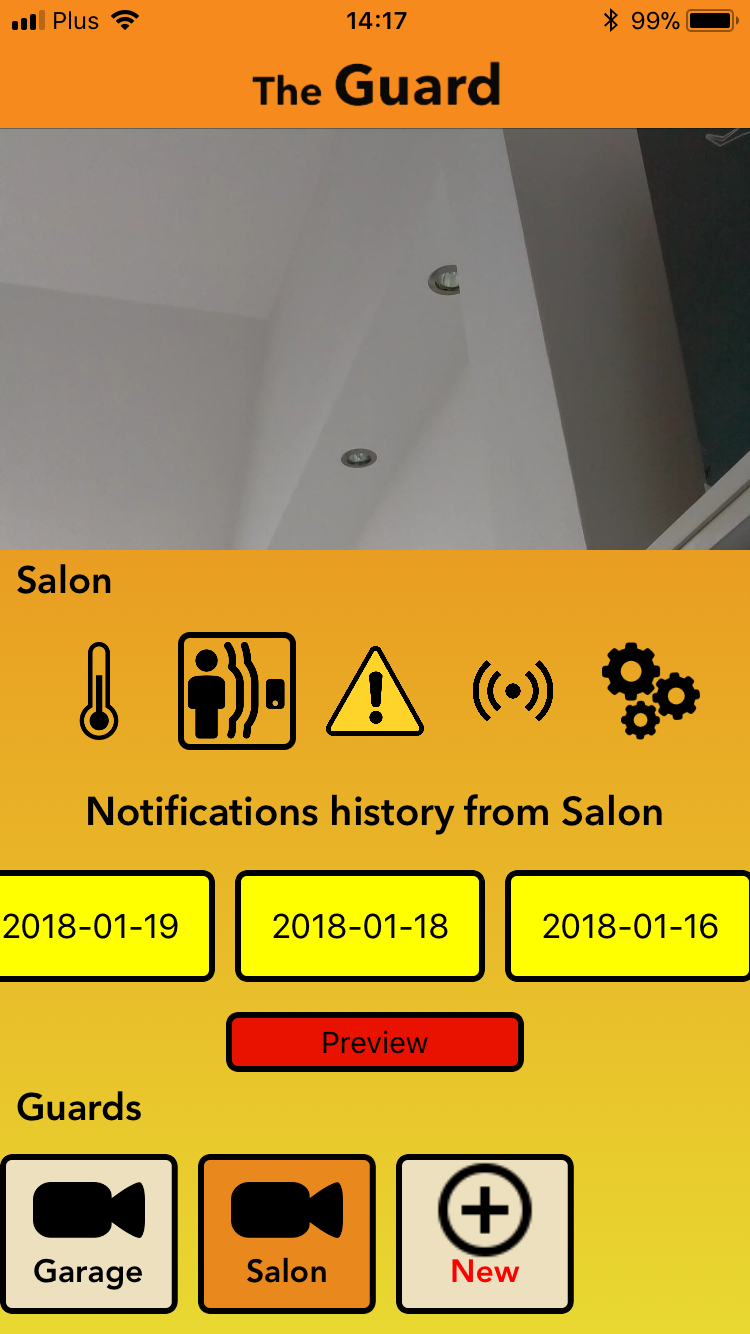
\includegraphics[width=\linewidth]{ios_screenshots/history.png}
    \caption{Sekcja historii notyfikacji  [źródło własne]}
    \label{img1}
\end{minipage}
\hspace{.05\linewidth}
\begin{minipage}{.4\linewidth}
    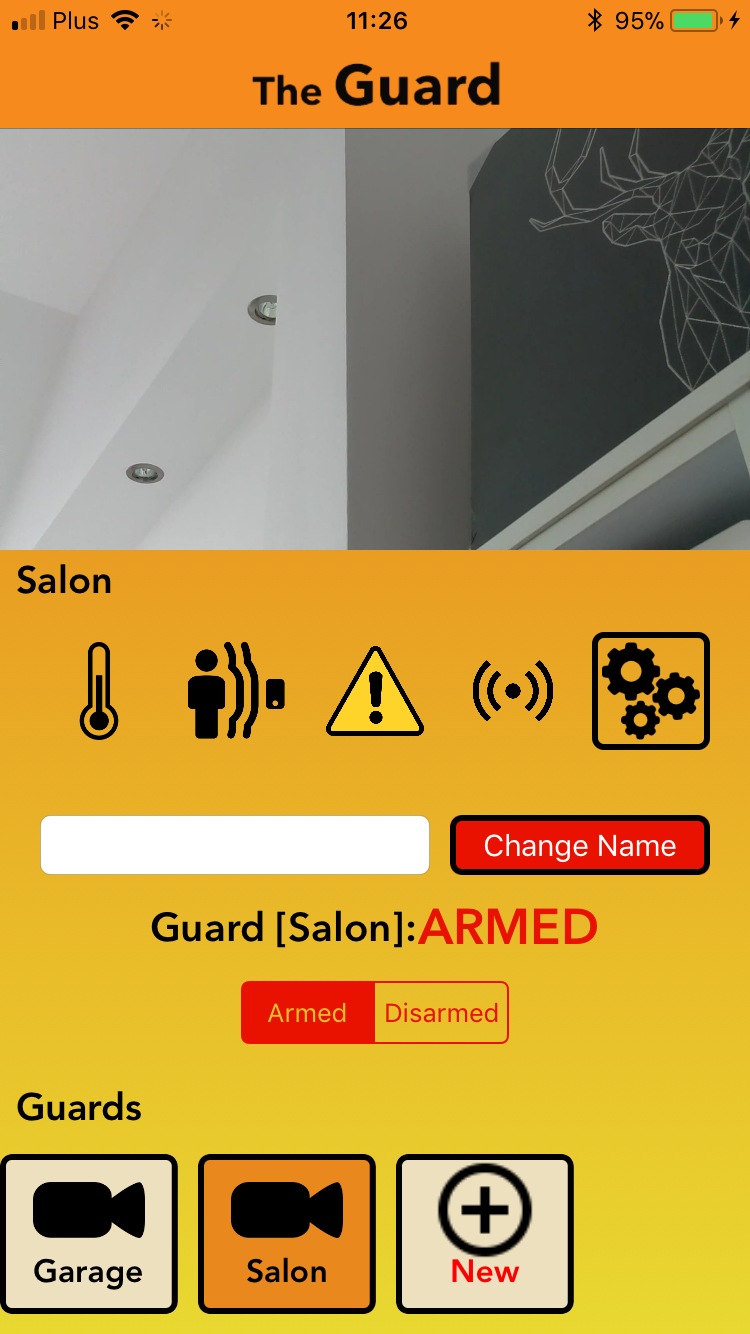
\includegraphics[width=\linewidth]{ios_screenshots/settings.png}
    \caption{Sekcja ustawień [źródło własne]}
    \label{img2}
\end{minipage}
\end{figure} 
\paragraph{Sekcja ustawień:}
Zrzut ekranu przedstawiono na rysunku (rys. x).
\paragraph{Sekcja monitoringu:}
Sekcja odpowiedzialna za prawidłowy odbiór obrazu z kamery zaznaczonej w dolnej części ekranu. Okno, w którym odbywa się stream ustawiono w taki sposób, aby bez względu na rozmiar telefonu utrzymywało proporcję 16:9. Pozbyto się dzięki temu czarnych ramek lub braku części obrazu ze streamu.

Przeprowadzono kilka testów aplikacji pod pełnym obciążeniem za pomocą programu Instruments. Szczególnie interesująco przedstawia się zużycie sieci podczas streamu obrazu. Widać, że w ciągu jednej minuty pobrano 6,61MB a wysłano jedynie 24,11Kb (rys. 5.8). Obraz pobierany jest tylko wtedy kiedy aplikacja jest aktywna. W ciągu godziny działania aplikacji pobierze ona około 400MB danych. Jednak dla zapewnienia komfortu użytkowania i płynnego streamu obrazu zalecane jest posiadanie łącza umożliwiającego transfer danych na poziomie min. 200KB/s. 
\begin{figure}[ht]
	\centering
	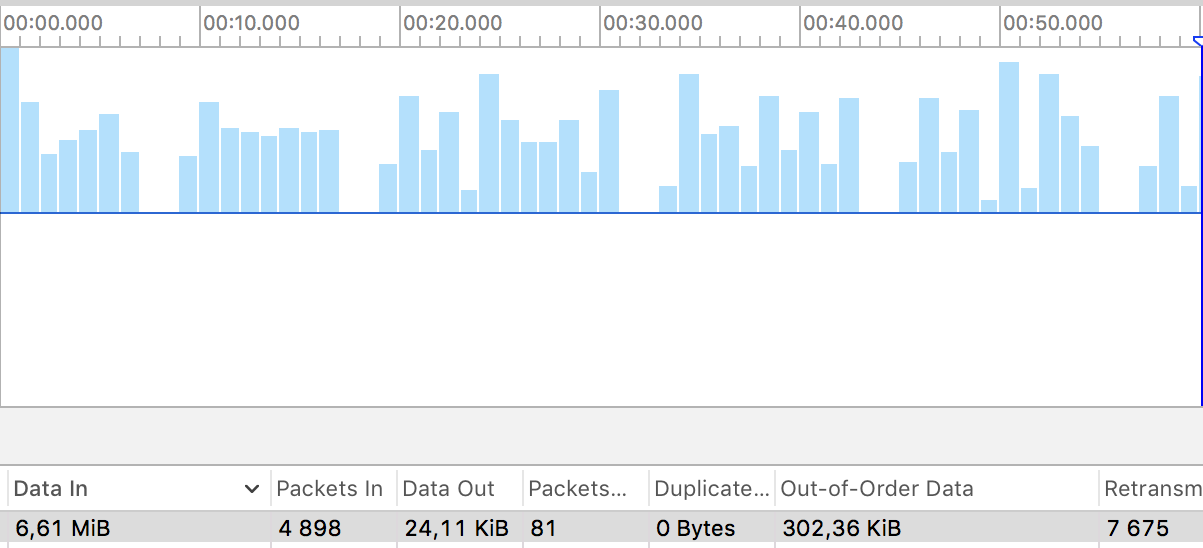
\includegraphics[width=11cm]{ios_screenshots/networkUsage.png}
	\caption{Zużycie sieci podczas streamu [źródło własne]}
\end{figure}
Przeprowadzono także test na zużycie pamięci RAM i zużycie procesora. Te jednak są niewielkie i wynoszą odpowiednio 25MB pamięci RAM i średnio 1 procent zużycia procesora.
Zużycie procesora wzrasta do poziomu ok. 15 procent tylko w momencie pobierania nagranego obrazu z serwera. Wtedy też zużycie pamięci RAM jest o około 5MB większe i wynosi około 30MB (rys. 5.9).
\begin{figure}[ht]
	\centering
	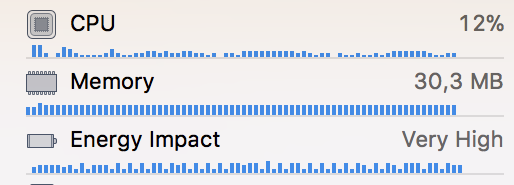
\includegraphics[width=11cm]{ios_screenshots/CPURAM.png}
	\caption{Zużycie procesora i RAM podczas największego obciążenia [źródło własne]}
\end{figure}
Testy przeprowadzono na iPhonie 6S i iPadzie Pro.


\section{Aplikacja internetowa}
Aplikacja webowa przeznaczona jest dla użytkowników wszystkich systemów operacyjnych i~została przetestowana w~przeglądarce Firefox. Rozmieszczenie komponentów aplikacji różni się od tego zastosowanego w~aplikacjach IOS oraz Android - spowodowane jest to inną rozdzielczością ekranu. 

\paragraph{Panel logowania / rejestracji użytkownika:}
\paragraph{Menu wyboru urządzenia:}
\paragraph{Główny panel aplikacji:}
\paragraph{Panel rejestracji urządzenia:}
\paragraph{Panel notyfikacji:}


\paragraph{Implementacja Django - połączenie z bazą danych:}
Biblioteka Django posiada wbudowane rozwiązania umożliwiające pobieranie informacji z bazy danych projektu dzięki czemu aplikacja webowa nie wysyła zapytań na określone dla aplikacji mobilnych porty, tylko komunikuje się bezpośrednio z bazą danych. Rozwiązanie to umożliwia uniezależnienie aplikacji webowej od stanu portów oraz zmniejsza liczbę potrzebnych zapytań wysyłanych do serwera.
Aplikacja internetowa przeznaczona jest dla użytkowników wszystkich systemów operacyjnych i~została przetestowana w~przeglądarce Firefox w systemach operacyjnych Microsoft Windows 10 oraz Linux Debian 9 (Firefox ESR 52.5.2 64 bit). Do stworzenia aplikacji użyto języków programowania Python 3, JavaScript oraz framework'u Django, natomiast frontend jest oparty na bibliotece Bootstrap oraz JQuery. Połączenie z~bazą danych Firebase zaimplementowano za pomocą Firebase Web Api. Rozmieszczenie komponentów aplikacji różni się od tego zastosowanego w~aplikacjach IOS oraz Android - spowodowane jest to inną rozdzielczością ekranu. 

\paragraph{Panel logowania / rejestracji użytkownika:} Panele logowania oraz rejestracji użytkownika są do siebie bardzo podobne - jedyna ich różnica jest w nazwie i~funkcjonalności. Obydwa panele składają się z~loga aplikacji oraz formularza w~którym trzeba podać adres email i~hasło. W przypadku panelu logowania, dane są weryfikowane i~jeśli są poprawne użytkownik zostaje zalogowany. Jeżeli użytkownik chce zarejestrować konto, sprawdzana jest poprawność adresu email, a następnie tworzone jest konto w usłudze FireBase Auth. W przypadku błędu, jest on wyświetlany powyżej formularza (rys. \ref{web_login})

\begin{figure}[ht]
	\centering
	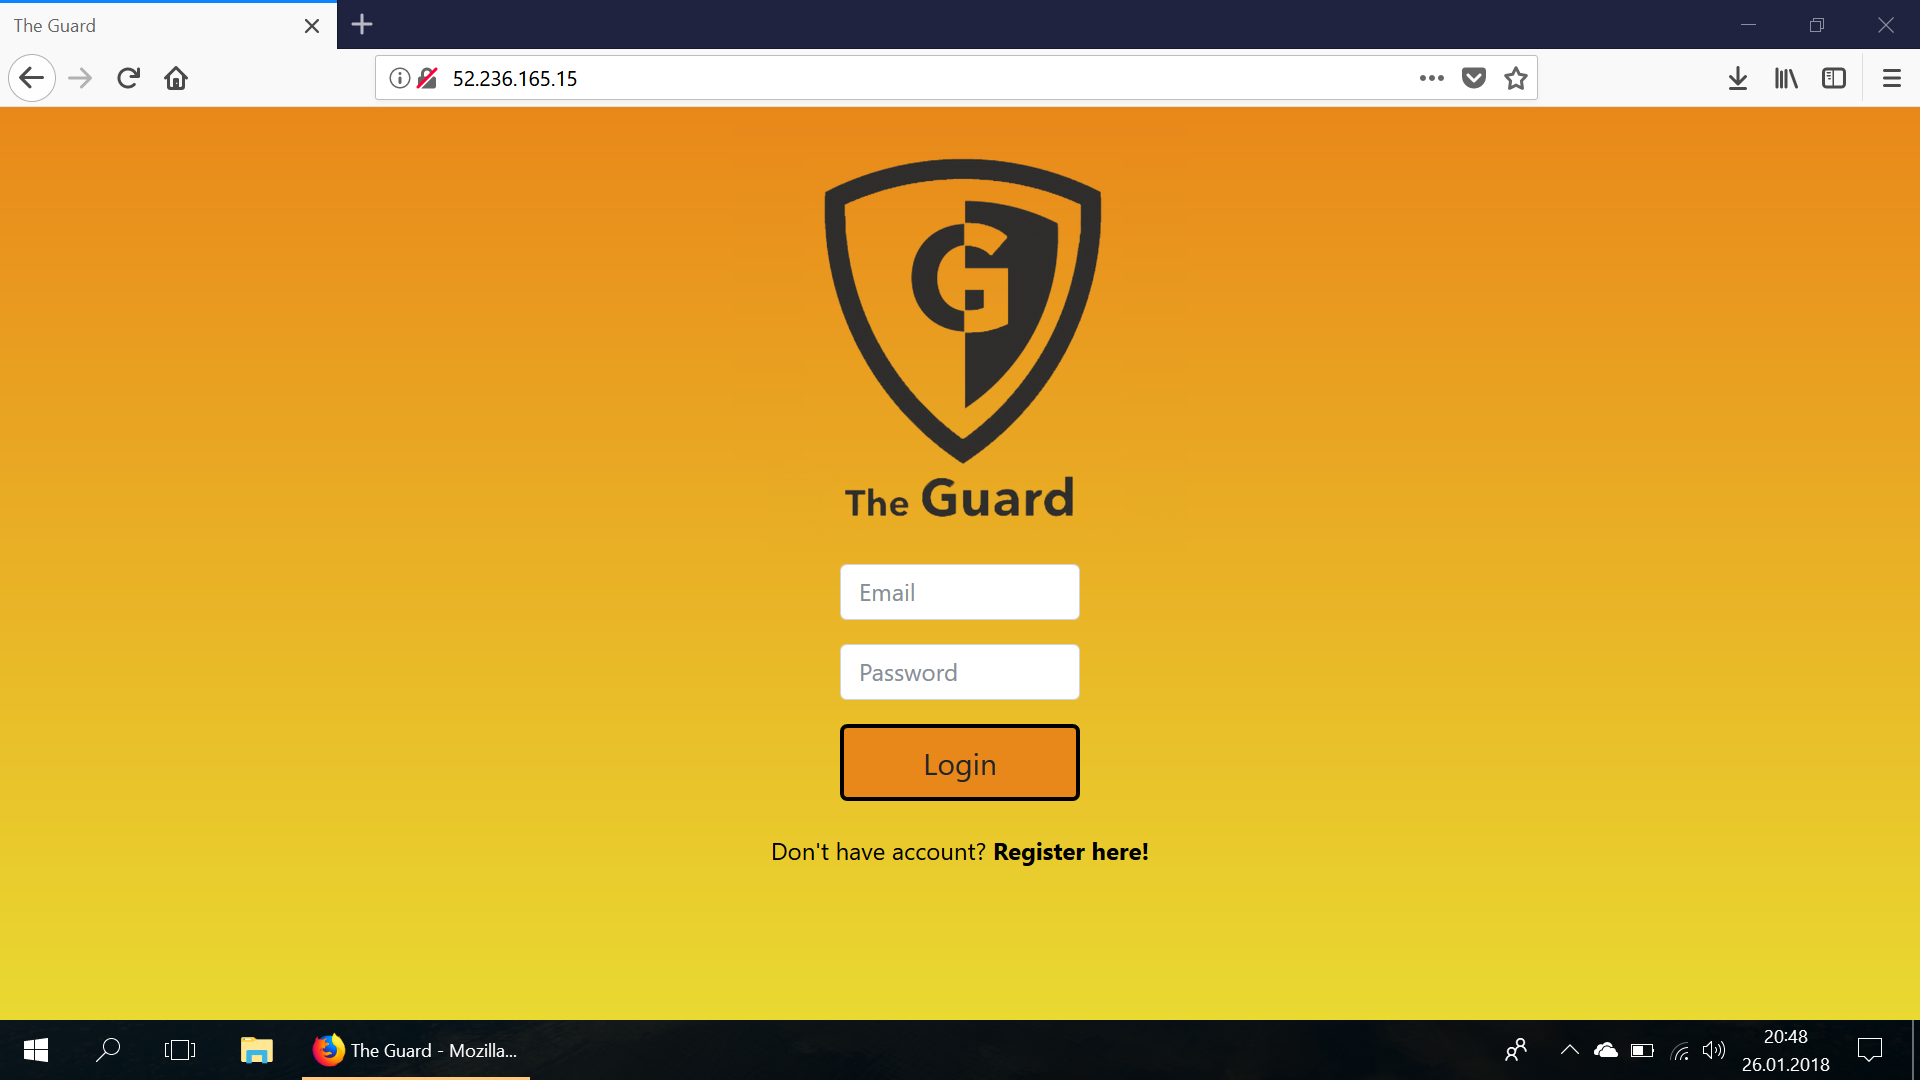
\includegraphics[width=9cm]{web_screenshots/login.png}
	\caption{Strona logowania w aplikacji webowej}
	\label{web_login}
\end{figure}

\begin{figure}[ht]
	\centering
	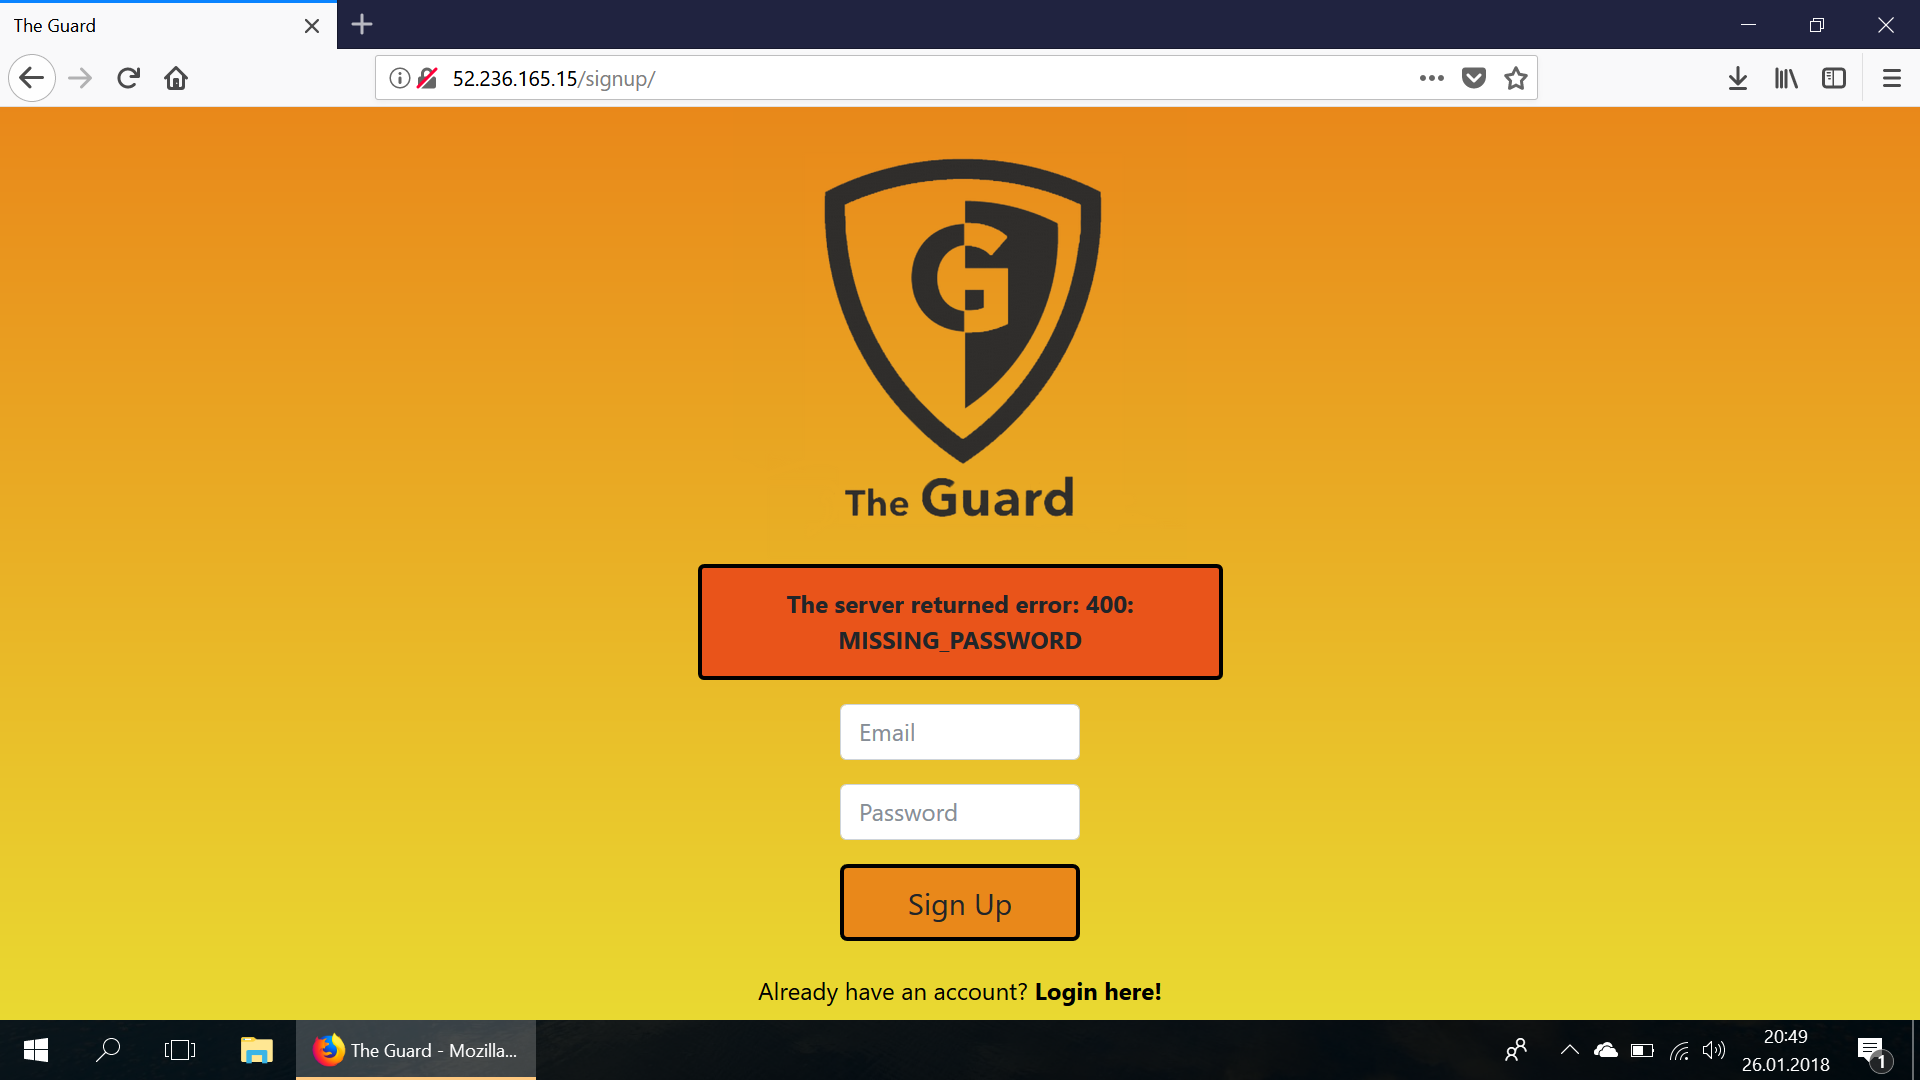
\includegraphics[width=9cm]{web_screenshots/error.png}
	\caption{Strona logowania - przykładowa obsługa błędu (użytkownik nie podał hasła)}
	\label{web_login_error}
\end{figure}
\paragraph{Menu wyboru urządzenia:} Po prawidłowym zalogowaniu do aplikacji, użytkownik może zobaczyć listę swoich urządzeń, dodać nowe oraz zaczyna dostawać powiadomienia w razie wykrytego zagrożenia. W~przypadku kliknięcia przycisku `Connect rasp', użykownik zostaje przekierowany do widoku umożliwiającego rejestrację nowego urządzenia(rys. \ref{web_register}). Po wprowadzeniu numeru seryjnego urządzenia oraz jego nazwy, zostaje dodany do baz danych. Po wybraniu urządzenia, informacje nt. jego stanu będą wyświetlane po prawej stronie okna, która w momencie zalogowania jest pusta (rys. \ref{web_main_page}). Urządzenia w~menu są rozpoznawane na podstawie ich nazw. 

\paragraph{Widok konkretnego urządzenia:} Po wybraniu z~menu kokretnego urządzenia, użytkownik zostaje przekierowany na stronę pojedyńczego urządzenia (rys. \ref{web_rasp_view}). Pod nazwą urządzenia i~jego numerem seryjnym wyświetlany jest aktualny obraz z kamery oraz stan czujników. Dzięki zastosowaniu nasłuchiwania na bazie danych Firebase, zmiany są na bieżąco wyświetlane na stronie. Użytkownik ma możliwość po naciśnięciu odpowiedniego przycisku:
\begin{itemize}
\item Zmienić nazwę urządzenia - po kliknięciu na przycisk rename znajdujący się obok nazwy urządzenia, użytkownik zostanie przekierowany do panelu zmiany nazwy (rys. \ref{web_rasp_rename}).
\item Wyłączyć / włączyć alerty 
\item Zobaczyć notyfikacje danego urządzenia - poprzez klknięcie na przycisk `Check notifications from this device', użytkownik zostanie przekierowany do widoku listy notyfikacji danego urządzenia (rys. \ref{web_rasp_notifications}).
\end{itemize}
\begin{figure}[ht]
	\centering
	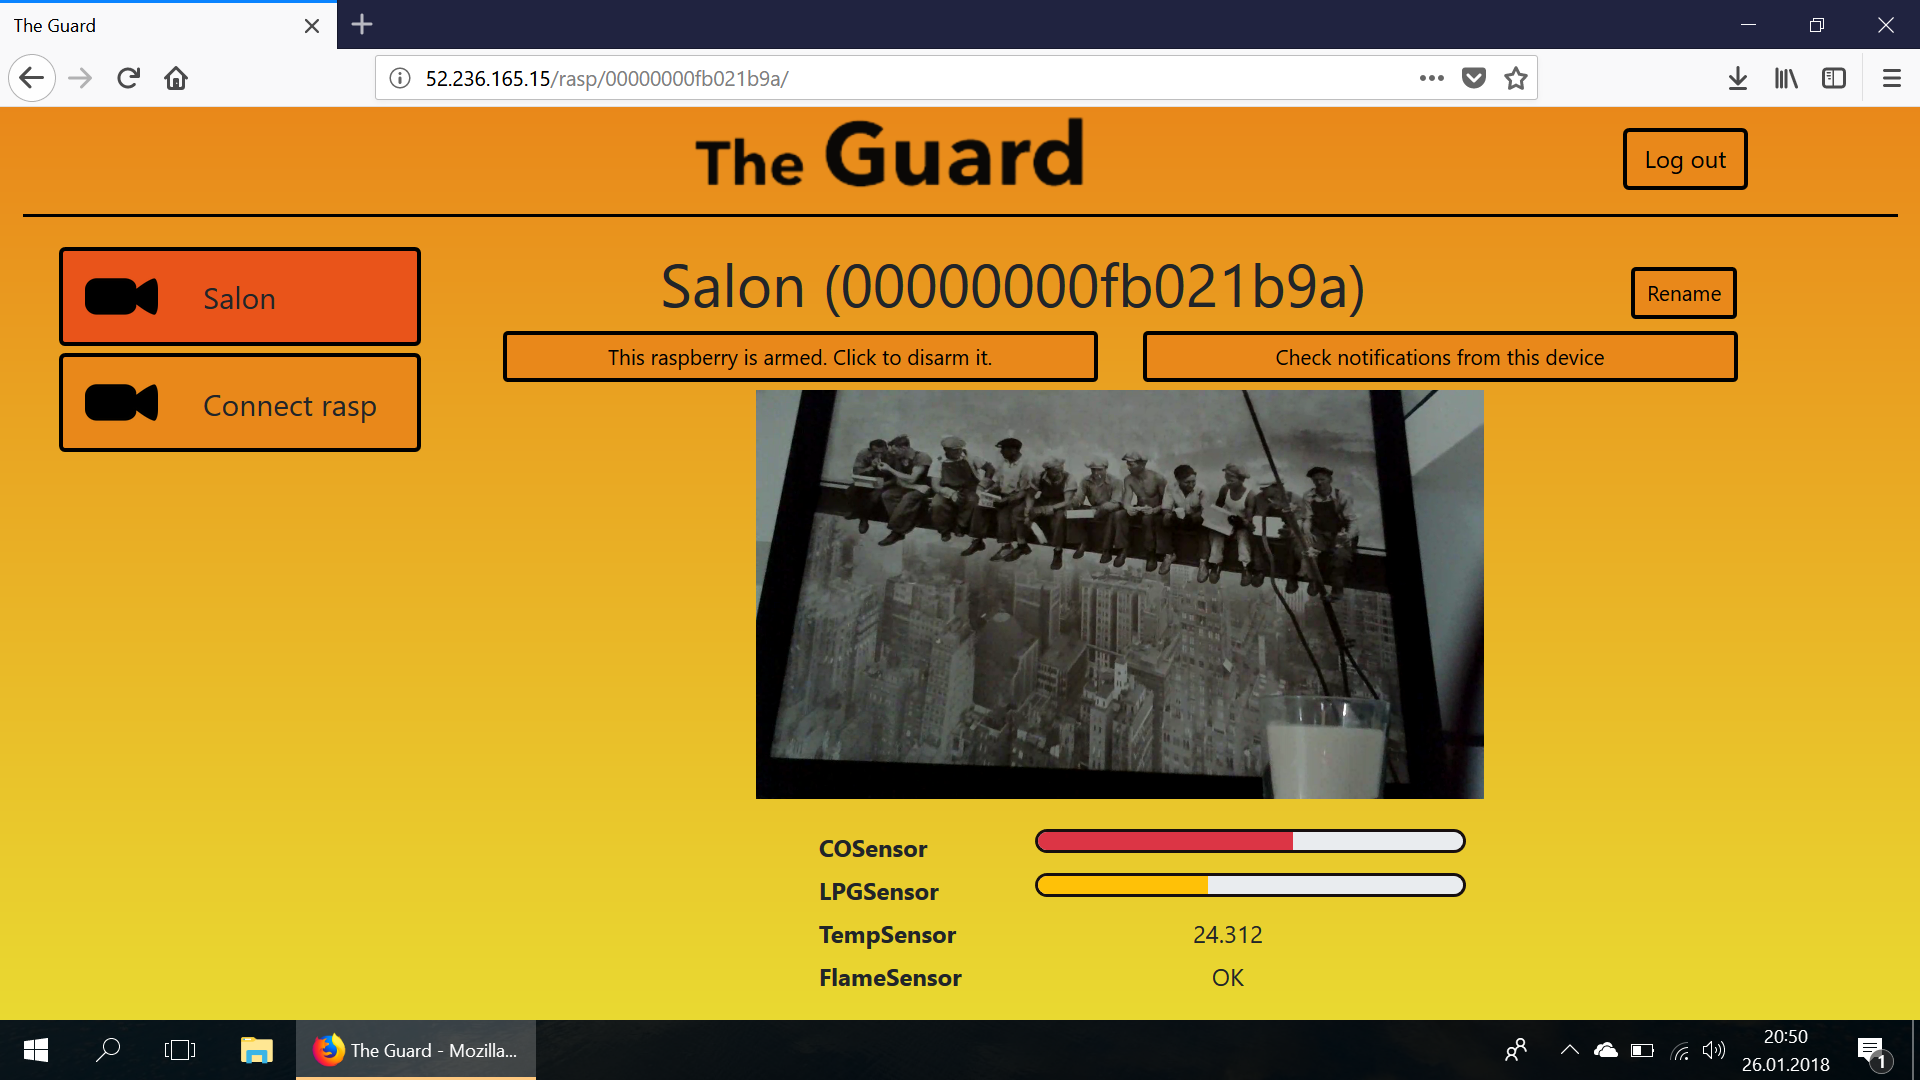
\includegraphics[width=9cm]{web_screenshots/rasp_view.png}
	\caption{Widok konkretnego urządzenia}
	\label{web_rasp_view}
\end{figure}
\begin{figure}[ht]
	\centering
	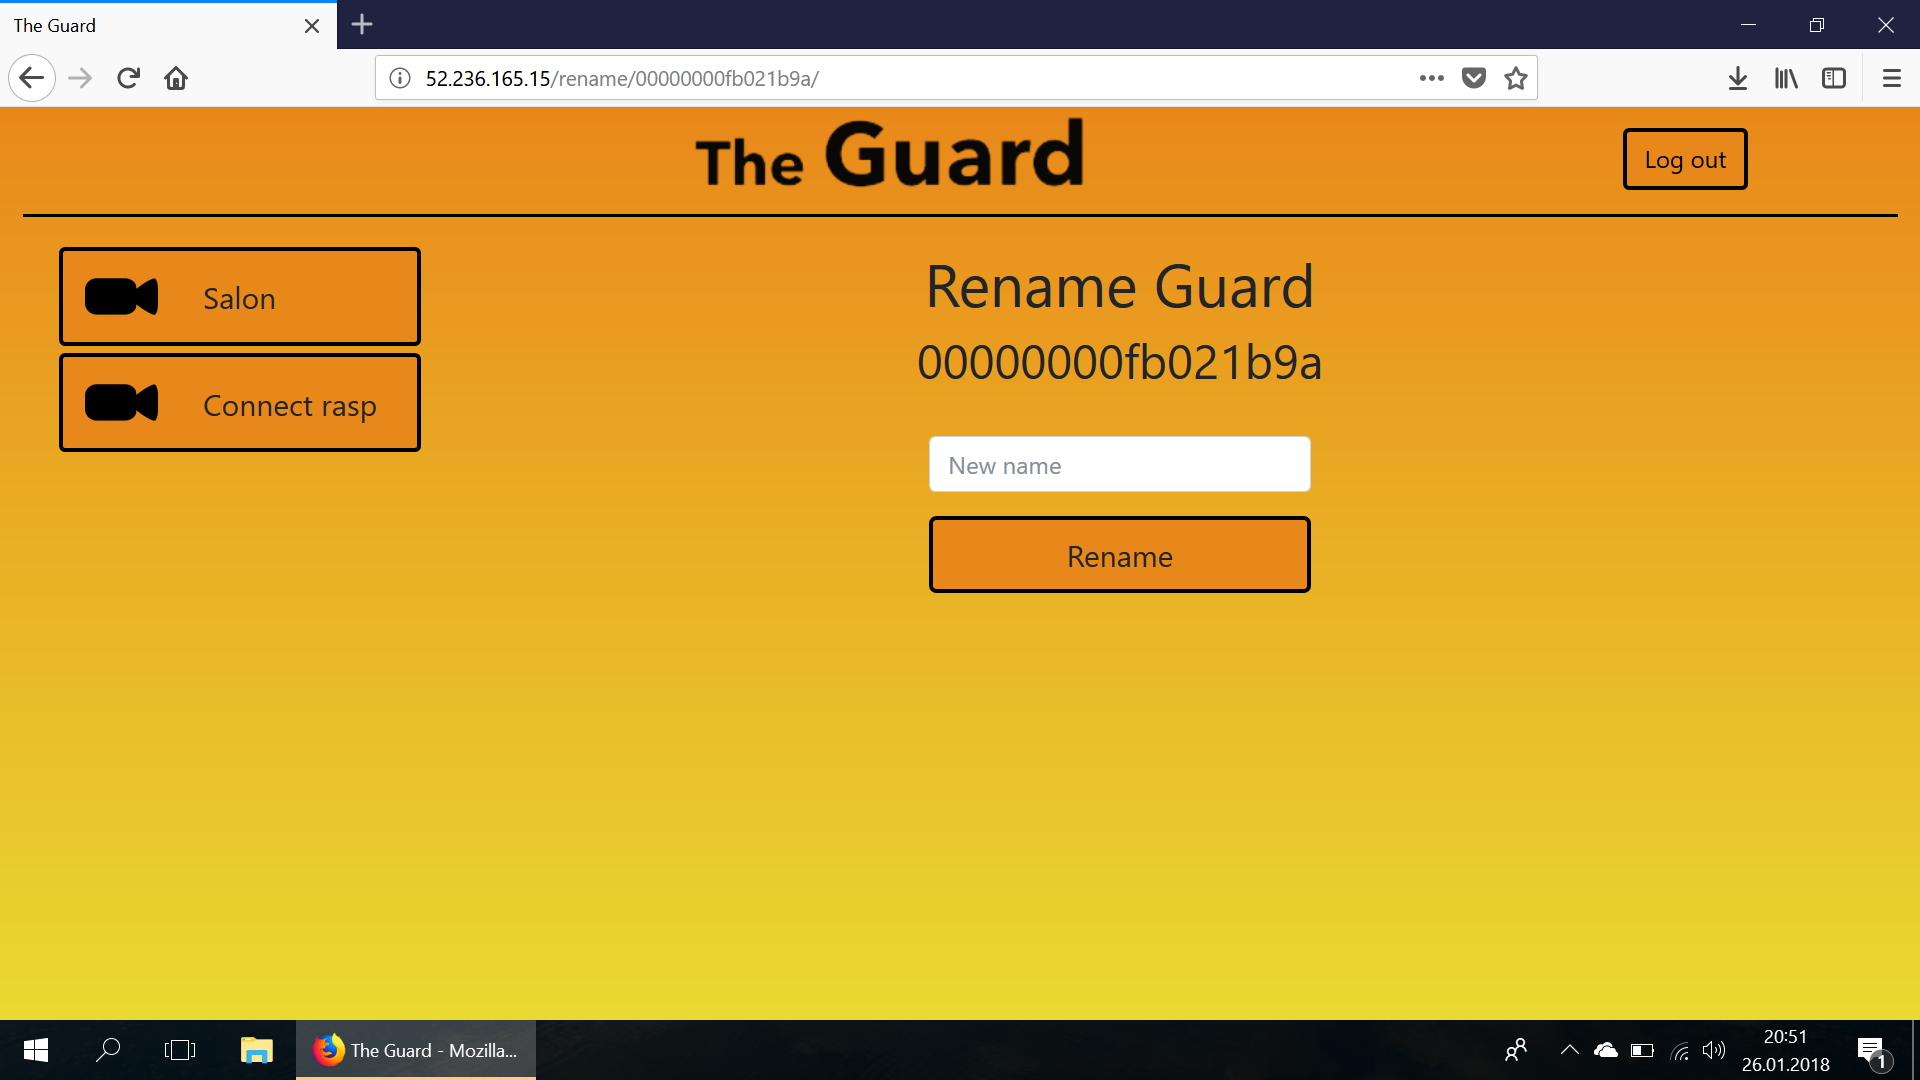
\includegraphics[width=9cm]{web_screenshots/rasp_rename.png}
	\caption{Panel zmiany nazwy urządzenia}
	\label{web_rasp_rename}
\end{figure}
\begin{figure}[ht]
	\centering
	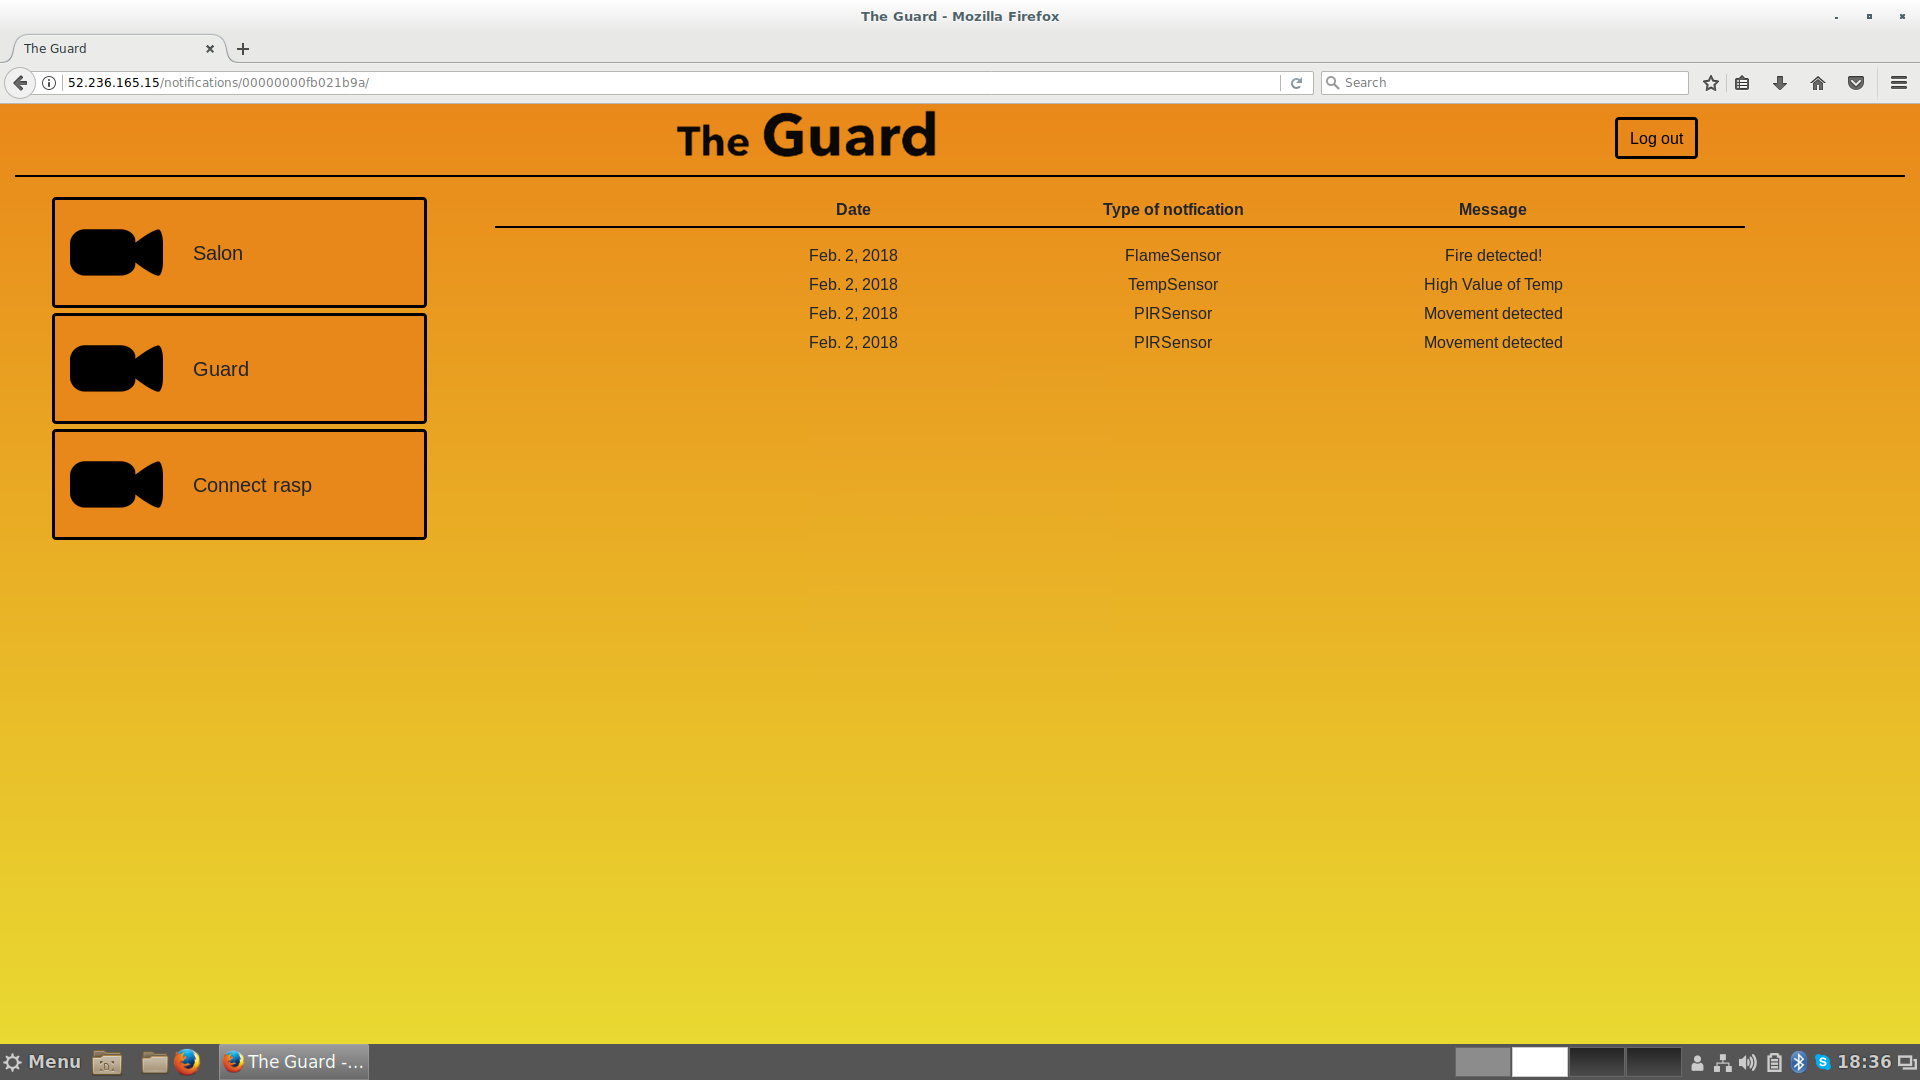
\includegraphics[width=9cm]{web_screenshots/rasp_notifications.png}
	\caption{Panel notyfikacji urządzenia}
	\label{web_rasp_notifications}
\end{figure}
\paragraph{Wyświetlanie notyfikacji:} W każdym z widoków aplikacji webowej w czasie rzeczywistym sprawdzane są notyfikacje z bazy danych z pomocą Firebase WebApi. W przypadku wykrycia zmiany uznawanej za niebezpieczną za pomocą skryptów przeglądarki (JavaScript + JQuery) wyświetlany jest monit informujący o niebezpiecznym zdarzeniu, co pokazane jest na rysunku \ref{web_rasp_notifications}.  

\paragraph{Implementacja Django - połączenie z bazą danych:}
Biblioteka Django posiada wbudowane rozwiązania umożliwiające pobieranie informacji z bazy danych projektu dzięki czemu aplikacja webowa nie wysyła zapytań na określone dla aplikacji mobilnych porty, tylko komunikuje się bezpośrednio z bazą danych. Rozwiązanie to umożliwia uniezależnienie aplikacji webowej od stanu portów oraz zmniejsza liczbę potrzebnych zapytań wysyłanych do serwera.
Aplikacja internetowa przeznaczona jest dla użytkowników wszystkich systemów operacyjnych i~została przetestowana w~przeglądarce Firefox w systemach operacyjnych Microsoft Windows 10 oraz Linux Debian 9 (Firefox ESR 52.5.2 64 bit). Do stworzenia aplikacji użyto języków programowania Python 3, JavaScript oraz framework'u Django, natomiast frontend jest oparty na bibliotece Bootstrap oraz JQuery. Połączenie z~bazą danych Firebase zaimplementowano za pomocą Firebase Web Api. Rozmieszczenie komponentów aplikacji różni się od tego zastosowanego w~aplikacjach IOS oraz Android - spowodowane jest to inną rozdzielczością ekranu. 

\paragraph{Panel logowania / rejestracji użytkownika:} Panele logowania oraz rejestracji użytkownika są do siebie bardzo podobne - jedyna ich różnica jest w nazwie i~funkcjonalności. Obydwa panele składają się z~loga aplikacji oraz formularza w~którym trzeba podać adres email i~hasło. W przypadku panelu logowania, dane są weryfikowane i~jeśli są poprawne użytkownik zostaje zalogowany. Jeżeli użytkownik chce zarejestrować konto, sprawdzana jest poprawność adresu email, a następnie tworzone jest konto w usłudze FireBase Auth. W przypadku błędu, jest on wyświetlany powyżej formularza (rys. \ref{web_login})

\paragraph{Menu wyboru urządzenia:} Po prawidłowym zalogowaniu do aplikacji, użytkownik może zobaczyć listę swoich urządzeń, dodać nowe oraz zaczyna dostawać powiadomienia w razie wykrytego zagrożenia. W~przypadku kliknięcia przycisku `Connect rasp', użykownik zostaje przekierowany do widoku umożliwiającego rejestrację nowego urządzenia(rys. \ref{web_register}). Po wprowadzeniu numeru seryjnego urządzenia oraz jego nazwy, zostaje dodany do baz danych. Po wybraniu urządzenia, informacje nt. jego stanu będą wyświetlane po prawej stronie okna, która w momencie zalogowania jest pusta (rys. \ref{web_main_page}). Urządzenia w~menu są rozpoznawane na podstawie ich nazw. 

\paragraph{Widok konkretnego urządzenia:} Po wybraniu z~menu kokretnego urządzenia, użytkownik zostaje przekierowany na stronę pojedyńczego urządzenia (rys. \ref{web_rasp_view}). Pod nazwą urządzenia i~jego numerem seryjnym wyświetlany jest aktualny obraz z kamery oraz stan czujników. Dzięki zastosowaniu nasłuchiwania na bazie danych Firebase, zmiany są na bieżąco wyświetlane na stronie. Użytkownik ma możliwość po naciśnięciu odpowiedniego przycisku:
\begin{itemize}
\item Zmienić nazwę urządzenia - po kliknięciu na przycisk rename znajdujący się obok nazwy urządzenia, użytkownik zostanie przekierowany do panelu zmiany nazwy (rys. \ref{web_rasp_rename}).
\item Wyłączyć / włączyć alerty 
\item Zobaczyć notyfikacje danego urządzenia - poprzez klknięcie na przycisk `Check notifications from this device', użytkownik zostanie przekierowany do widoku listy notyfikacji danego urządzenia (rys. \ref{web_rasp_notifications}).
\end{itemize}

\paragraph{Wyświetlanie notyfikacji:} W każdym z widoków aplikacji webowej w czasie rzeczywistym sprawdzane są notyfikacje z bazy danych z pomocą Firebase WebApi. W przypadku wykrycia zmiany uznawanej za niebezpieczną za pomocą skryptów przeglądarki (JavaScript + JQuery) wyświetlany jest monit informujący o niebezpiecznym zdarzeniu, co pokazane jest na rysunku \ref{web_rasp_notifications}.  

\paragraph{Implementacja Django - połączenie z bazą danych:}
Biblioteka Django posiada wbudowane rozwiązania umożliwiające pobieranie informacji z bazy danych projektu dzięki czemu aplikacja webowa nie wysyła zapytań na określone dla aplikacji mobilnych porty, tylko komunikuje się bezpośrednio z bazą danych. Rozwiązanie to umożliwia uniezależnienie aplikacji webowej od stanu portów oraz zmniejsza liczbę potrzebnych zapytań wysyłanych do serwera.
